\section{Implementierung Prototyp}
\label{sec:implementierung}

Nachdem im letzten Abschnitt eine Festlegung auf spezifischen Kriterien zur Erhebung von Messwerten vorgenommen wurde, folgt eine detaillierte Beschreibung der Implementierung des zu erstellenden Prototypen. Der komplette Quellcode sowie alle zugehörigen Konfigurationsdateien befinden sich in einem Github-Repository unter folgender Url \url{https://github.com/derMacon/stack-scale-benchmark} .

\subsection{Schichtenmodell \checkmark}
Der Arbeitsfluss der Anwendung wurde in Abbildung \ref{fig:stackOverview} visuell dargestellt. Die unterschiedlichen Komponenten wurden dabei in vier verschiedene Schichten eingeteilt: 

\begin{figure}[ht!]
	\centering
	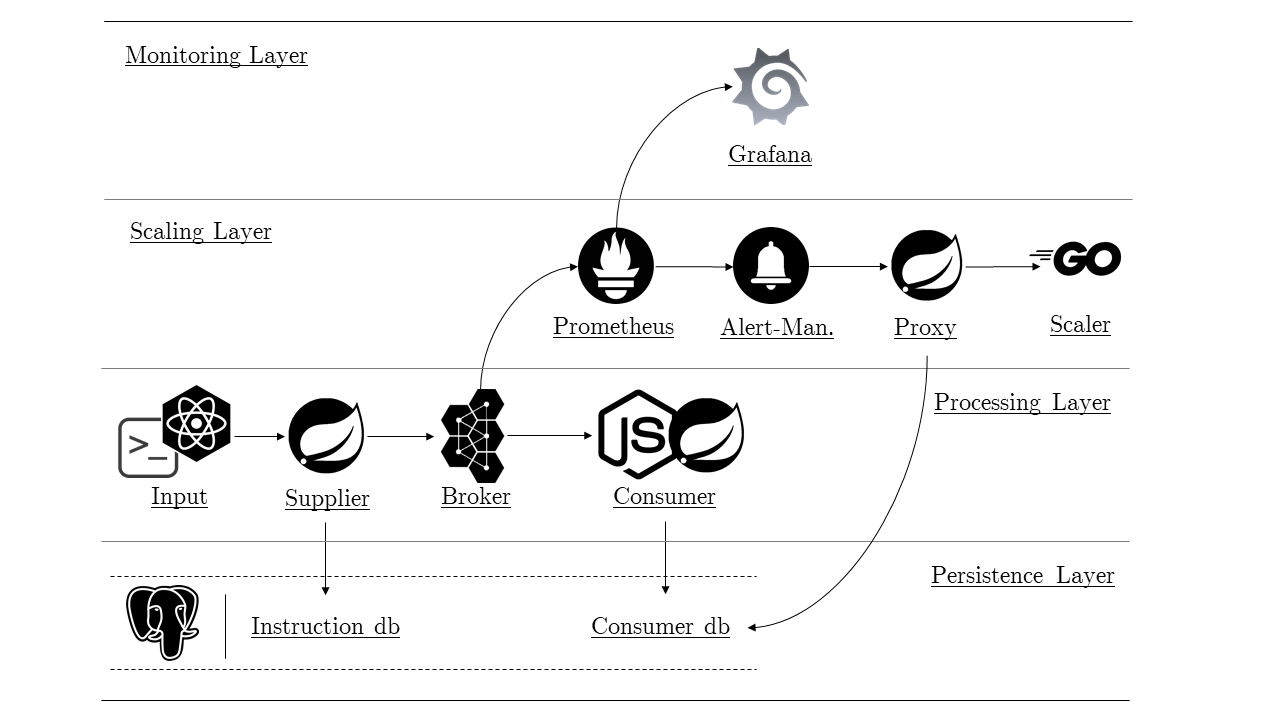
\includegraphics[width=\linewidth]{kapitel/problemloesung/implementierung/_img/overview-bw}
	\caption[Komponenten-Stack im Überblick]{Komponenten-Stack im Überblick}
	\label{fig:stackOverview}
\end{figure}

\begin{itemize}
  \item Persistenzschicht (engl. \emph{persistence layer}): Beinhaltet sämtliche Komponenten, die für das Abspeichern gegebener Datensätze in dazugehörige Datenbanken zuständig sind. Um Nebenläufigkeit zu ermöglichen wird hier ebenfalls auf Schnittstellen über einen Message-Broker zurückgegriffen. Eine Manipulation der Daten findet auf dieser Ebene nicht statt.
  \item Verarbeitungsschicht (engl. \emph{processing layer}): Beinhaltet sämtliche Komponenten, die für die direkte Verarbeitung der Business-Logik zuständig sind. Die Kommunikation zwischen den Komponenten findet über eine REST-Schnittstelle sowie einen Message-Broker statt. Der Message-Broker stellt hierbei vor allem eine nebenläufige Verarbeitung der konsumierenden Komponenten sicher. Allerdings bietet dieser ebenfalls die Schnittstelle zur Skalierungsschicht (engl. \emph{scaling layer}).
  \item Skalierungsschicht (engl. \emph{scaling layer}): Beinhaltet sämtliche Komponenten zum Skalieren der konsumierenden Komponenten. Hierbei wird auf eine universelle Schnittstelle des Message Broker zurückgegriffen um entsprechende Metriken abzugreifen, die für die Evaluierung hinterlegter Regeln zur Skalierung verwendet werden. Ansonsten wird in Komponenten dieser Schicht das Zeitverhalten des Initialisierungsprozesses der konsumierenden Komponenten überwacht und an Schnittstellen der Persistenzschicht weitergeleitet.
  \item Monitoring Ebene: Diese Schicht besteht aus einer einzigen Komponente, deren Aufgabe es ist erhaltene Daten visuell darzustellen. Um einen zeitlichen Überblick zu geben, werden die Daten intern vom Werkzeug gespeichert. Da es sich um lokal verwaltete Datensätze handelt, die für den Rest der Applikation keinerlei Bedeutung darstellen, wurde verzichtet eine Lösung zu finden, in der diese ebenfalls in einer Komponente der Persistenzschicht abzuspeichern.
\end{itemize}

\subsection{Komponenten im Überblick \checkmark}
Es folgt eine kurze Zusammenfassung der Funktionalität sowie der Anforderungen an die jeweiligen Komponenten.

\subsubsection{Input \checkmark}
Um es dem Benutzer zu ermöglichen, gezielte Messwerte zu erfassen, wird eine REST-Schnittstelle vom System bereitgestellt. Es ist zwar möglich, dass der Benutzer selbstständig Anfragen für diese Schnittstelle generiert und absendet, beabsichtigt ist allerdings, dass der Benutzer auf vordefinierte Skripte oder eine entsprechende Benutzeroberfläche zurückgreift. Die Benutzeroberfläche ist sehr funktional gehalten, sodass es zwar möglich ist, hierüber Anfragen an das System zu stellen, dennoch empfiehlt sich gerade für komplexere Anfrageszenarien der Gebrauch der bereitgestellten Bash-Skripte. Bezüglich der Skripte gibt es ebenfalls diverse Abstraktionsschichten. So ist es zum Beispiel möglich, mithilfe einer definierten Grammatik Anforderungen zu definieren, die sich beliebig kombinieren lassen. Hierzu wurden mehrere vordefinierte Dateien angelegt, deren Inhalt über ein entsprechendes Skript an das Backend geschickt werden kann. Allerdings gibt es weitere Skripte, die auf diesem Prozess aufsetzen und somit eine Abstraktionsschicht aufbauen, sodass sich der Endbenutzer hiermit nicht auseinandersetzen muss.

\subsubsection{Supplier \checkmark}
Diese Komponente ist in der Lage, die vereinfachten Anfragen des Benutzers zu interpretieren und in Nachrichten umzuwandeln, die vom System verarbeitet werden können. Hierbei werden bereits an dieser Stelle der Verarbeitungspipeline diverse Informationen an die ursprüngliche Nachricht angeheftet, um im späteren Verlauf entsprechende Metriken zu berechnen. Außerdem erfolgt eine erste Kommunikation mit der Persistenzschicht, in der die übersetzten Benutzeranfragen abgespeichert werden. Hierbei wird direkt auf die Datenbank zugegriffen, da im System lediglich eine Singleton-Instanz des \emph{Suppliers} vorhanden ist. Zwar unterstützt die verwendete Postgres-Datenbank mehrere Klienten zur gleichen Zeit, nativ ist diese Anzahl jedoch begrenzt und muss angemessen konfiguriert werden. Des Weiteren stellt die Supplier-Komponente zwei Modi hinsichtlich der Geschwindigkeit bereit, in der Nachrichten an den Broker übermittelt werden. So ist es zum Beispiel möglich, Nachrichten über einen gewissen Zeitraum hinweg abzuschicken oder aber eine Transaktion zu bilden, in der alle auf einmal geschickt werden.

\subsubsection{Broker \checkmark}
Ein Message-Broker stellt die Funktionalität bereit, Nachrichten über ein gegebenes Protokoll an mehre Konsumenten zu vermitteln. Hierzu wurde eine Implementierung von Apache namens "\emph{Active MQ\footnote{\url{https://github.com/apache/activemq}}}" gewählt. Diese besitzt zwei Betriebsmodi, einmal das Arbeiten mit einer \emph{Topic} sowie mit einer \emph{Queue}. Eine Topic stellt ein \emph{Publisher-Subscriber-Muster} bereit, in dem alle eingehenden Nachrichten an alle registrierten Konsumenten verschickt werden \cite[Seite~33 ff.]{activemq-snyder}. Demgegenüber steht eine \emph{Queue} (Warteschlange), die eingehende Nachrichten lediglich an einen einzelnen Konsumenten übermittelt, wobei der Broker hierbei als eine Art Load Balancer\footnote{Erklärung \emph{Load Balancer} siehe Abschnitt \ref{sec:loadbalancer}} agiert. Bevor die Nachrichten jedoch aus einer der beiden Datenstrukturen entfernt werden, muss der betreffende Konsument eine \emph{Acknowledgement-Nachricht} an den Broker schicken, um zu signalisieren, dass die Nachricht nicht nur angenommen, sondern auch korrekt verarbeitet werden konnte. Es gilt weiterhin noch hervorzuheben, dass die eingeschriebenen Konsumenten bei neuen Nachrichten stets benachrichtigt werden und es clientseitig keine Logik braucht, um zum Beispiel event- oder intervallbasiert eine Abfrage an den Broker zu steuern. Da diese Komponente ebenfalls den Einstiegspunkt für das Monitoring System \emph{Prometheus} (siehe Abschnitt \ref{ss:prometheus}) darstellt, benötigt der Broker eine Schnittstelle über die er diesem Tool Messdaten zur Verfügung stellen kann. Die von ActiveMq bereitgestellt Schnittstelle nennt sich "\emph{Java Management Extension API (JMX)}" und ist die Standard-API zur Verwaltung von Java Applikationen \cite[Seite~331 ff.]{activemq-snyder}.


\subsubsection{Consumer \checkmark}
Die konsumierenden Komponenten können beliebig skaliert werden und implementieren die in Abschnitt \ref{ss:fiktiverWorkflow} definierten Arbeitsschritte. Hierbei wird auf diverse Libraries zurückgegriffen, wobei die restliche Logik eher schlicht gehalten wurde. Die Komponenten kommunizieren lediglich über den Message-Broker mit dem Nachrichten-Supplier und über einen weiteren Nachrichten-Broker mit der Persistenzschicht um die extrahierten Elemente abzulegen.


\subsubsection{Prometheus \checkmark}
\label{ss:prometheus}
"\emph{Prometheus is an open source systems monitoring and alerting toolkit}" \cite[Seite~400]{oreillyPrometheus}. Es ist möglich über eine definierte Anfragensprache Daten Dritter zu verarbeiten. Diese Daten können über ein einfaches Textformat von den Komponenten ausgegeben werden. Es ist möglich dieses Textformat händisch zu schreiben, allerdings wird in der Praxis vermehrt auf Libraries, die auf den Client zugeschnitten wurden, gesetzt. Prometheus ist unter der Apache 2.0 Lizenz veröffentlicht \footnote{https://github.com/prometheus/prometheus}, und wurde primär in der Programmiersprache Go implementiert. Das intervallbasierte Anfragen (engl. "\emph{scrapen}") der Metriken wird von der Prometheus-Komponente selbst durchgeführt, die zu überwachenden Komponenten müssen sich selbst nicht darum kümmern Daten an Prometheus zu übermitteln.

\todo{checken ob Figure am Ende immer noch nicht unter die folgenden Absatz auf Seite passt, ggf. aendern}
\begin{figure}[ht!]
	\centering
	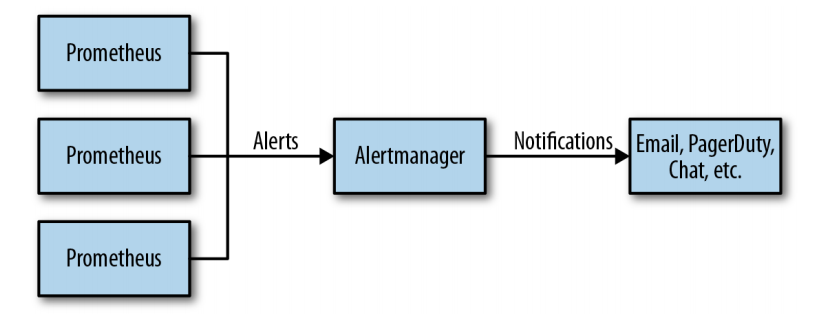
\includegraphics[width=.8\linewidth]{kapitel/problemloesung/implementierung/_img/alert-man-p291}
	\caption[Alert Manager - Übersicht]{Alert Manager - Übersicht \cite[Seite~291]{oreillyPrometheus}}
	\label{fig:alertManOverview}
\end{figure}

\subsubsection{Alert Manager \checkmark}
"\emph{Alerting is one of the components of monitoring, allowing you to notify a human when there is a problem}" \cite[Seite~291]{oreillyPrometheus}. Prometheus bietet hierbei die Möglichkeit mithilfe der funktionalen Anfragesprache \emph{PromQl} diverse Bedingungen zu definieren unter denen dies geschehen soll. Da es in einer produktiven Containerumgebung durchaus möglich ist, dass mehrere Prometheus-Instanzen parallel arbeiten, wurde das Benachrichtigen in eine weitere Komponente (den \emph{Alert Manger}) ausgelagert. Dieser synchronisiert, sammelt und gruppiert die Alerts der verschiedenen Prometheus-Instanzen und sendet Benachrichtigungen an definierte Nachrichtenkanäle, die sich beispielsweise aus einem Emailpostfach, einer Pagernachricht oder Chatnachricht auf Plattformen wie Slack zusammensetzen können (siehe Abbildung \ref{fig:alertManOverview}).


\subsubsection{Scaler Proxy \checkmark}
Diese Komponente bietet eine REST-Schnittstelle, die im Alert-Manager hinterlegt wird. Sobald eine der Regeln anschlägt, wird der Aufruf an diese Komponente weitergeleitet. Im Endeffekt dient diese Komponente lediglich als Proxy-Service, da ihre primäre Aufgabe darin besteht diese Nachricht an eine weitere Komponente weiterzuleitet. In einer produktiven Umgebung würde diese Komponente komplett enfallen, da es möglich ist den Alert-Manager derartig zu konfigurieren, dass er direkt die öffentlichen Schnittstellen der Scaler-API anspricht. Es wurde sich dennoch für das Zwischenschalten eines solchen Proxy-Services entschieden um genauere Messwerte zu erhalten. Gerade hinsichtlich der Initialisierungsphasen von Containern ist es angebracht so kurz vorher wie möglich einen Timestamp zu setzen. Da es keine Möglichkeit gibt direkt in die Konfiguration der Scaler-Api einzugreifen ist diese Lösung der nächstbeste Ansatz. Sobald eine Skalierungsanfrage weitergeleitet wurde, wird diese noch unbeantwortete Anfrage intern in einer Datenstruktur abgelegt. Sobald ein entsprechender Container komplett initialisiert wurde, ruft dieser eine weitere Schnittstelle des Proxy-Services auf. Daraufhin wird ein \emph{Acknowledgement-Timestamp} in der hinterlegten Anfrage gesetzt und an die Persistenzschicht weitergeleitet. 

Außerdem bietet diese Komponente die Möglichkeit für den Benutzer direkt Exemplare eines Consumers hochzufahren. Die verwendete Schnittstelle dient als Umgehung des herkömmlichen Programmflusses und wird zur Generierung der skalierungsschichtenunabhängigen Metrikberechnung verwendet (siehe Abschnitt \ref{par:specContainer}). Über dedizierte Endpunkte können diese Metriken als .csv Datei ausgelesen werden. 


\subsubsection{Scaler \checkmark}
"\emph{The goal of the Docker Scaler project is to provide a REST HTTP interface to scale services and nodes}"\cite{docker-scaler}. Außerdem werden mit jeder Skalierungsanfrage Statusinformationen über die aktuelle sowie zukünftige Anzahl von Instanzen des zu skalierenden Services zurückgegeben, die es dem Proxy-Service ermöglichen davon ausgehend einen Skalierungsstop für neue Anfragen beizubehalten oder aufzuheben. Dieser ist nötig damit das System keine weiteren Skalierungsprozesse starten, wenn bereits aktive Skalierungen vorgenommen werden.


\subsubsection{Grafana \checkmark}
Wenn es zum Alert durch den Alert Manager kommt, wird in einer Produktivumgebung der Erste Schritt sein die Performanz des Systems durch dedizierte Dashboard zu überprüfen \cite[Seite~97]{oreillyPrometheus}. Grafana ist ein Werkzeug, das dies über eine Weboberfläche direkt im Browser ermöglicht. Es bietet die Möglichkeit Graphen, Tabellen und weitere Visualisierungskomponenten zu erstellen um zum Beispiel die Latenzzeit oder CPU Auslastung zu überprüfen. Diese Metriken können für das ganze System oder nur einen Teil generiert werden. Es ist das bevorzugte Visualisierungswerkzeug für Prometheus, bietet allerdings ebenfalls Unterstützung für verschiedene weitere Systeme wie zum Beispiel \emph{Graphite}, \emph{Elasticsearch} oder \emph{PostgreSQL}.


\subsubsection{Mock scaler api \checkmark}
Diese Komponente ist nicht Kernbestandteil des Komponenten-Stacks. Sie dient lediglich während der Entwicklungszeit dazu die Scaler-Api zu emulieren. So ist es zum Beispiel möglich lokal eine Instanz des Scaler-Proxy Projekts in einer beliebigen IDE als Standard Spring Projekt auszuführen. Sämtliche Skalierungs-Anfragen können von dieser Komponente angenommen werden, da sie auf dem gleichen Port wie der "\emph{echte}" Scaler läuft, wobei sie dabei ebenfalls in der Lage ist diverse Rückgabenachrichten an den Klienten zu übergeben.




\subsection{Input \checkmark}

Der Benutzer besitzt die Möglichkeit, sowohl über eine Benutzeroberfläche als auch über Bash-Skripte Benchmark Anfragen an das System zu stellen. Im Folgenden wird beides im Detail erläutert.

\subsubsection{Bash \checkmark}
\paragraph{Aufbau}
In der folgenden Abbildung ist der Aufbau des Bash-Projektes dargestellt. Der Benutzer besitzt drei Möglichkeiten, Anfragen an das System zu stellen. Für jeden Einstiegspunkt wurde ein entsprechendes Bash-Skript zur Verfügung gestellt.

\begin{figure}[ht!]
	\centering
	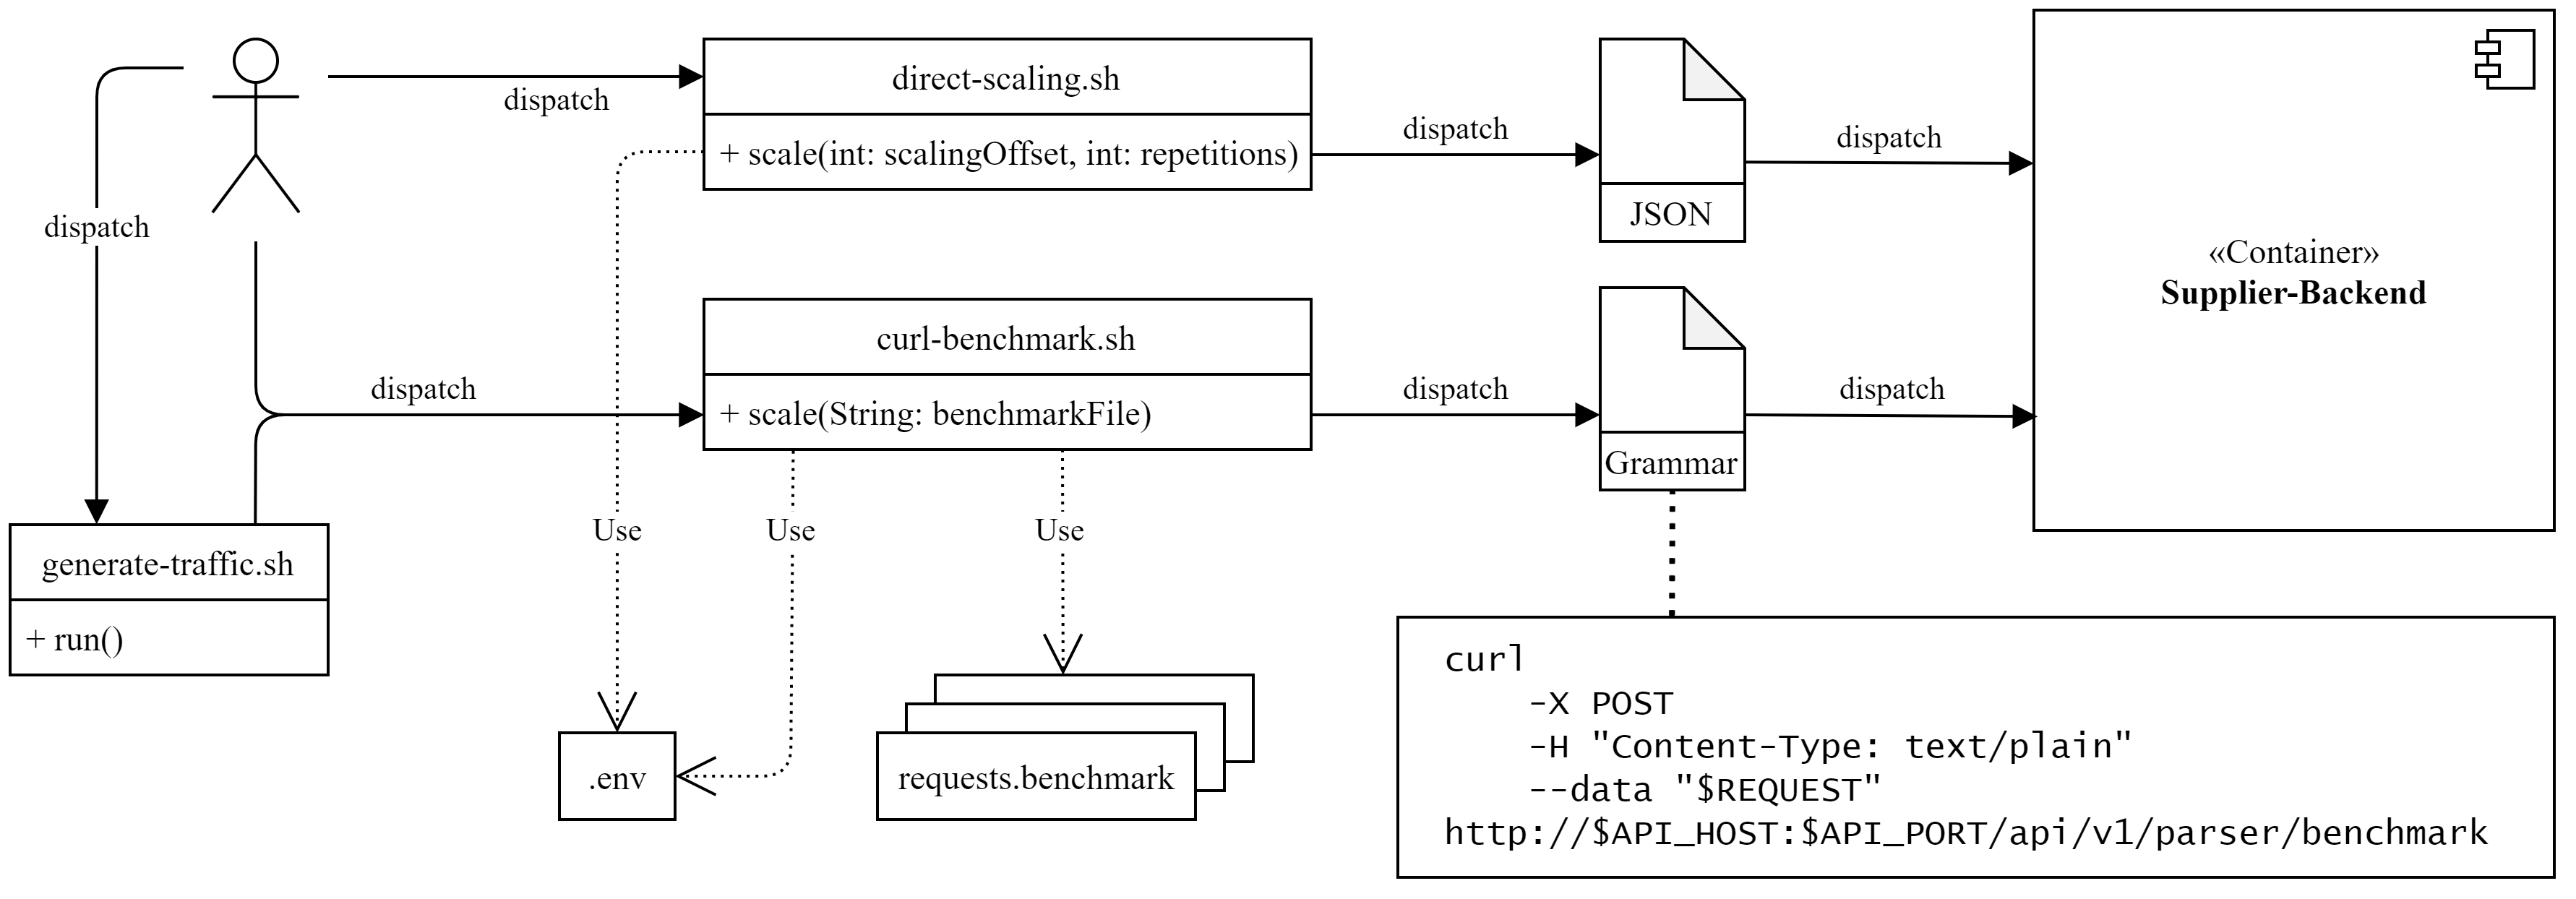
\includegraphics[width=\linewidth]{kapitel/problemloesung/implementierung/_img/input-uml}
	\caption[Bash Input UML]{Bash Input UML}
	\label{fig:bashOverview}
\end{figure}

\begin{itemize}
  \item \emph{direct-scaling.sh}: bietet die Möglichkeit eine direkte Skalierungsanfrage an das System zu senden, ohne Payment-Messages verwenden zu müssen. Als Parameter werden die Skalierungsanzahl sowie die Wiederholungen erwartet (genauere Erklärung siehe \ref{erklaerungDirScal}).
  \item \emph{curl-benchmark.sh}: sendet eine Skalierungsanfrage mit dem Dateiinhalt einer Datei, dessen Pfad als Eingabeparameter verarbeitet wird. Die Datei besitzt die Dateiendung \emph{.benchmark}, wobei der Inhalt einer spezifizierten Grammatik folgt (siehe \ref{lst:instruction-grammar}).
  \item \emph{generate-traffic.sh}: dient als vereinfachter Einstiegspunkt für den Benutzer. Hierbei werden rekursiv alle verfügbaren \emph{.benchmark} Dateien der Directory und übergibt diese der Reihe nach dem \emph{curl-benchmark} Skript.
\end{itemize}

Im folgenden Listing (siehe \ref{verb:scriptStruct}) ist ein Auszug der Projekt-Struktur abgebildet. Neben den genannten Skripts sind sämtliche \emph{.benchmark} Dateien nach Services in Unterordner aufgeteilt worden. Die \emph{.env} Datei beinhaltet die Verbindungsdaten zum Komponenten-Stack. Diese müssen bei der ersten Ausführung vom Benutzer angeglichen werden. Im Wesentlichen beschränkt sich dies auf die IP-Adresse des Systems, falls der Benutzer in der Stack-Konfiguration entsprechende Änderungen vornimmt, sind diese an dieser Stelle ebenfalls zu vermerken.

\label{verb:scriptStruct}
\begin{minipage}{\linewidth}
\begin{lstlisting}[caption={Bash Skript - Struktur},style=bashStyle]
  $ tree request-scripts/ -a -L 3 --charset=ascii
  request-scripts/
  |-- curl-benchmark.sh
  |-- direct-scaling.sh
  |-- .env
  |-- generate-traffic.sh
  |-- README.md
  `-- requests
      |-- mixed
      |   |-- benchmark_large_mixed.benchmark
      |   |-- benchmark_medium_mixed.benchmark
      |   `-- benchmark_small_mixed.benchmark
      ...
\end{lstlisting}
\end{minipage}

\label{erklaerungDirScal}
\paragraph{Manuelles Skalieren}
Hierfür wird auf ein Bash-Skript namens "\emph{direct-scaling}" zurückgegriffen. Das Skript nimmt zwei Parameter entgegen. Der Erste beschreibt die Anzahl der Instanzen, zu der das System skaliert werden soll, wobei hierbei eine inkrementelle Erhöhung von einer Instanz pro Durchlauf durchgeführt wird. Der zweite Parameter gibt die Wiederholungen dieser testweisen Skalierung an. Der Aufruf \verb+./direct-scaling.sh 10 20+ resultiert beispielsweise darin, das sowohl für den Node.js als auch Spring Boot Service jeweils 10 Skalierungsschritte durchgeführt werden. Wenn zum Beispiel bereits ein Node.js-Container läuft, wird im ersten Test eine weitere Instanz angefordert. Sobald die beiden Instanzen verfügbar sind, wird der Alert-Manager durch die Prometheus-Komponente angewiesen die überflüssige Instanz zu löschen. Sobald wieder ein einziger Container läuft, wird dieser Schritt neunzehn weitere Male wiederholt. Anschließend erfolgt die nächste Skalierung bei der nun zwei neue Container kreiert werden sollen, anstatt wie vorher nur ein weiterer. Auch hier folgen 20 Wiederholungen. Diese Schritte werden solange durchgeführt bis zehn Container zwanzig Mal instanziiert wurden.

\label{lst:direct-scaling}
\begin{minipage}{\linewidth}
\begin{lstlisting}[caption={direct-scaling},style=bashStyle]
...

request() {
  curl "http://$HOST:$DIRECT_SCALING_PORT/manual-scale?additionalCnt=$1&service=$4"
}

node_request() {request $1 $2 $3 'NODE'}
spring_request() {request $1 $2 $3 'SPRING'}

for scalingOffset in $(seq 1 $1)
do 
  for curr_rep in $(seq 1 $2)
	do 
    node_request $scalingOffset $curr_rep $2
    spring_request $scalingOffset $curr_rep $2
  done
done
\end{lstlisting}
\end{minipage}
\paragraph{Skalieren mithilfe von Grammatik}
Das beschriebene Skript sowie der zugrunde liegende Http-Endpunkt bieten eine Möglichkeit, das Skalieren als Reaktion auf unbeantwortete Nachrichten zu umgehen. Um jedoch einen herkömmlichen Testdurchlauf zu starten, greift der Benutzer auf einen Endpunkt vom \emph{Supplier} zurück: 

\begin{verbatim}
  curl 
    -X POST 
    -H "Content-Type: text/plain" 
    --data "$REQUEST" 
    "http://$API_HOST:$API_PORT/api/v1/parser/benchmark"
\end{verbatim}

Es handelt sich hierbei um eine POST-Anfrage. Im Body wird der Dateiinhalt eines für diesen Zweck verfassten Skripts angeheftet. Im Projekt wurden diverse Beispiele verfasst. Diese liegen im Ordner \emph{./requests} und tragen die Dateiendung "\emph{.benchmark}". Der Inhalt korrespondiert zu einer spezifizierten Grammatik (siehe Listing \ref{lst:instruction-grammar}).

\label{lst:instruction-grammar}
\begin{verbatim}
  request     := batch*
  batch       := serviceName { instruction | instruction,* };
  serviceName := SPRING | NODE
  instruction := BENCHMARK ( messageCnt, duration ) | WAIT ( duration )
  messageCnt  := [0-9]+
  duration    := [0-9]+
\end{verbatim}

Es können beliebig viele Batchanfragen den Anfragenbody angeheftet werden. Eine Batch stellt in diesem Zusammenhang eine Gruppe an Skalierungsanfragen an einen bestimmten Service dar, wobei diese mindestens eine Skalierungsinstruktion enthalten müssen. In diesem System gibt es zwei wesentliche Skalierungsinstruktionen: 

\begin{enumerate}
  \item BENCHMARK: Nimmt zwei Parameter entgegen. Der erste spezifiziert, wie viele neue Instanzen erstellt werden sollen, während der Zweite angibt, über welchen Zeitraum dies geschehen soll. Alle numerischen Angaben müssen einen positiven Ganzzahlwert enthalten. Da das System selbstständig in der Lage sein soll diese Instanzen wiederum auf ein gesetztes Minimum zu minimieren, wurde sich aktiv dagegen entschieden, das Herunterskalieren in die Grammatik aufzunehmen, um dem Benutzer eine möglichst schlicht gehaltene Schnittstelle zur Verfügung zu stellen.
  \item WAIT: Diese Instruktion erwartet lediglich einen einzigen Parameter, der angibt wie viele Millisekunden gewartet werden soll, bevor die nächste Instruktion dem System übergeben wird. 
\end{enumerate}


Damit der Benutzer allerdings direkt Anfragen ausführen kann, ohne sich mit der Grammatik beschäftigen zu müssen, wurde ein weiterer Skript-Aufsatz 
für das \emph{curl-benchmark} Skript entwickelt. Dieses trägt den Namen "\emph{generate-traffic.sh}" und sucht rekursiv absteigend in der eigenen Directory nach Dateien mit der entsprechenden Endung. Anschließend werden diese Skripte an das \emph{curl-benchmark} der Reihe nach als Parameter übergeben.

\paragraph{Benutzeroberfläche}
Die Benutzeroberfläche wurde mithilfe des Javascript-Frameworks \emph{React.js} entwickelt. Es ist möglich über diverse Select-Felder die voreingestellten Pfad, sowie Payment Optionen auszuwählen. Außerdem ist es möglich, die Anzahl sowie die Zeitspanne der Anfrage zu spezifizieren. Beim Initialisierungsprozess dieses Projekts starten zuallererst alle dargestellten React-Komponenten. React.js ist ein komponentenbasiertes Framework, hierbei werden sämtliche visuellen Elemente als einzelne Komponenten betrachtet, wobei es möglich ist diese Komponenten zu gruppieren und somit neue Komponenten zu formen. Außerdem ermöglicht das Framework diesen Komponenten einen sogenannten \emph{State} anzuheften, in dem Daten hinterlegt werden können. Wenn diese an irgendeiner Stelle modifiziert werden, erkennt React dies und rendert die betroffene Komponente sowie alle untergeordneten Komponenten neu. Dies ist insbesondere hilfreich um die Formulareinträge direkt abzuspeichern. Bei der Initialisierung versucht die Frontend-Komponente die darzustellenden Optionen vom \emph{Supplier} zu fetchen. Dieser beantwortet diese Anfrage mit den Daten, die im Anschluss in der Oberfläche angezeigt werden. Wenn der Benutzer darauf folgend Daten auswählt beziehungsweise Daten in die Felder einträgt, werden hierfür zugeschnittene Eventhandler-Funktionen ausgelöst. Diese Eventhander registrieren die Datenauswahl und speichern sie direkt im State der Komponente ab. Wenn der Benutzer nun auf den Button zum Absenden der Anfrage klickt, muss hierbei lediglich der State ausgelesen werden und an die entsprechende Backend-Api-Schnittstelle geschickt werden. In Abbildung \ref{fig:reactUi} wurde hierfür der aktuelle Stand der Oberfläche dargestellt.

\begin{figure}[ht!]
	\centering
	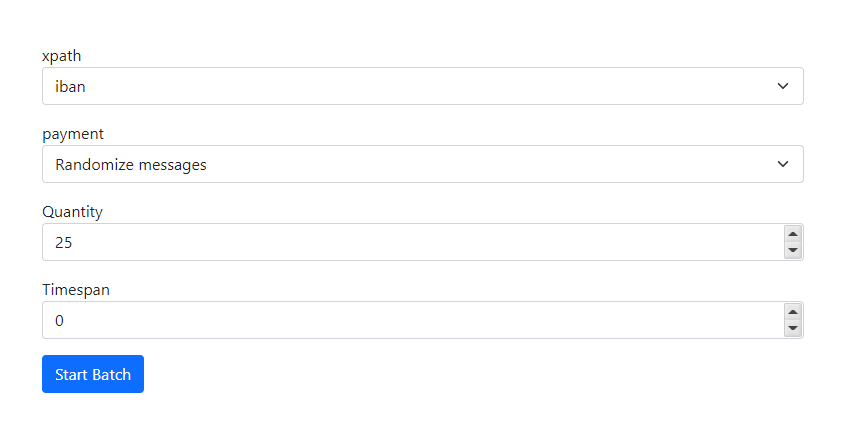
\includegraphics[width=.9\linewidth]{kapitel/problemloesung/implementierung/_img/react01}
	\caption[React - Benutzeroberfläche]{React - Benutzeroberfläche}
	\label{fig:reactUi}
\end{figure}

Während der Entwicklungszeit des restlichen Systems, wurde das Arbeiten mit der Benutzeroberfläche allerdings vermehrt zum Flaschenhals. Sobald ein neues Feature oder ein neuer Datensatz in eine Anfrage integriert wurde oder sich das zugrunde liegende Datenmodell änderte, war es jedes Mal ein großer Aufwand dies ebenfalls in der Oberfläche anzupassen. Da die vorher spezifizierte Grammatik sowie die zugrunde liegende API einen deutlich flexibleren Ansatz und eine komplexere Ablauflogik ermöglichen wurde sich bereits relativ früh in der Entwicklung dagegen entschlossen diesen Ansatz der grafischen Benutzerführung weiterzuverfolgen. Die Oberfläche dient hierbei eher als ein \emph{Proof of concept} um darzustellen, wie ein solches Projekt konfiguriert werden muss. Da dem skriptbasierten Ansatz dieselben API-Schnittstellen zugrunde liegen wie dem oberflächenbasierten Ansatz, ist es ohne Probleme möglich das aktuelle React-Projekt den überarbeiteten Gegebenheiten anzupassen, falls dies in Zukunft gewünscht sein sollte.


\subsection{Supplier Backend}
Bei dieser Komponente handelt es sich um ein Spring Projekt, dessen Aufgabe es ist, Benutzeranfragen in Nachrichten zu übersetzen, die vom System interpretiert und verarbeitet werden können. Die Schnittstelle für den Benutzer besteht hierbei aus einer REST-Api, die über Tools wie zum Beispiel curl angesprochen werden kann.

\subsubsection{Implementierung}

\paragraph{Generelle Spring Projektübersicht \checkmark}
Da diese Komponente bezüglich der Struktur eines Spring-Projekts alle wesentlichen Merkmale besitzt, wird die genutzte Projektstruktur an dieser Stelle etwas näher erläutert. 

\label{verb:supplierStruct}
\begin{minipage}{\linewidth}
\begin{lstlisting}[caption={Supplier Backend - Struktur},style=bashStyle]
  $ tree stack/supplier-backend/ -a -L 7 --charset=ascii
  stack/supplier-backend/
  |-- Dockerfile
  |-- pom.xml
  `-- src
      `-- main
          |-- java
          |   `-- dps
          |       `-- hoffmann
          |           `-- producer
          |               |-- config
          |               |-- controller
          |               |-- model
          |               |-- properties
          |               |-- repository
          |               |-- response
          |               |-- service
          |               `-- SupplierBackendApplication.java
          `-- resources
              |-- application-dev.properties
              |-- application-prod.properties
              `-- application.properties
\end{lstlisting}
\end{minipage}

Das Muster, nach dem sämtliche Komponenten des Komponenten-Stacks entwickelt wurden, wird als \emph{Layered Architecture Pattern} oder \emph{n-tier pattern} bezeichnet \cite{oreilly-layered-arch}. Es stellt einen weitverbreiteten Standard in Java Enterprise Applikationen dar und zeichnet sich durch die klare Unterteilung der verschiedenen Hierarchien aus (siehe Abbildung \ref{fig:layeredArchitecture}). Sämtliche Packages innerhalb der Spring-Projekte finden sich innerhalb einer der Schichten wieder. Es sei ebenfalls hervorzuheben, dass sämtliche Schichten stets nur mit ihren direkt angrenzenden Schichten kommunizieren. Dies stellt ein weitaus übersichtlicheres Design sicher.

\begin{figure}[ht!]
	\centering
	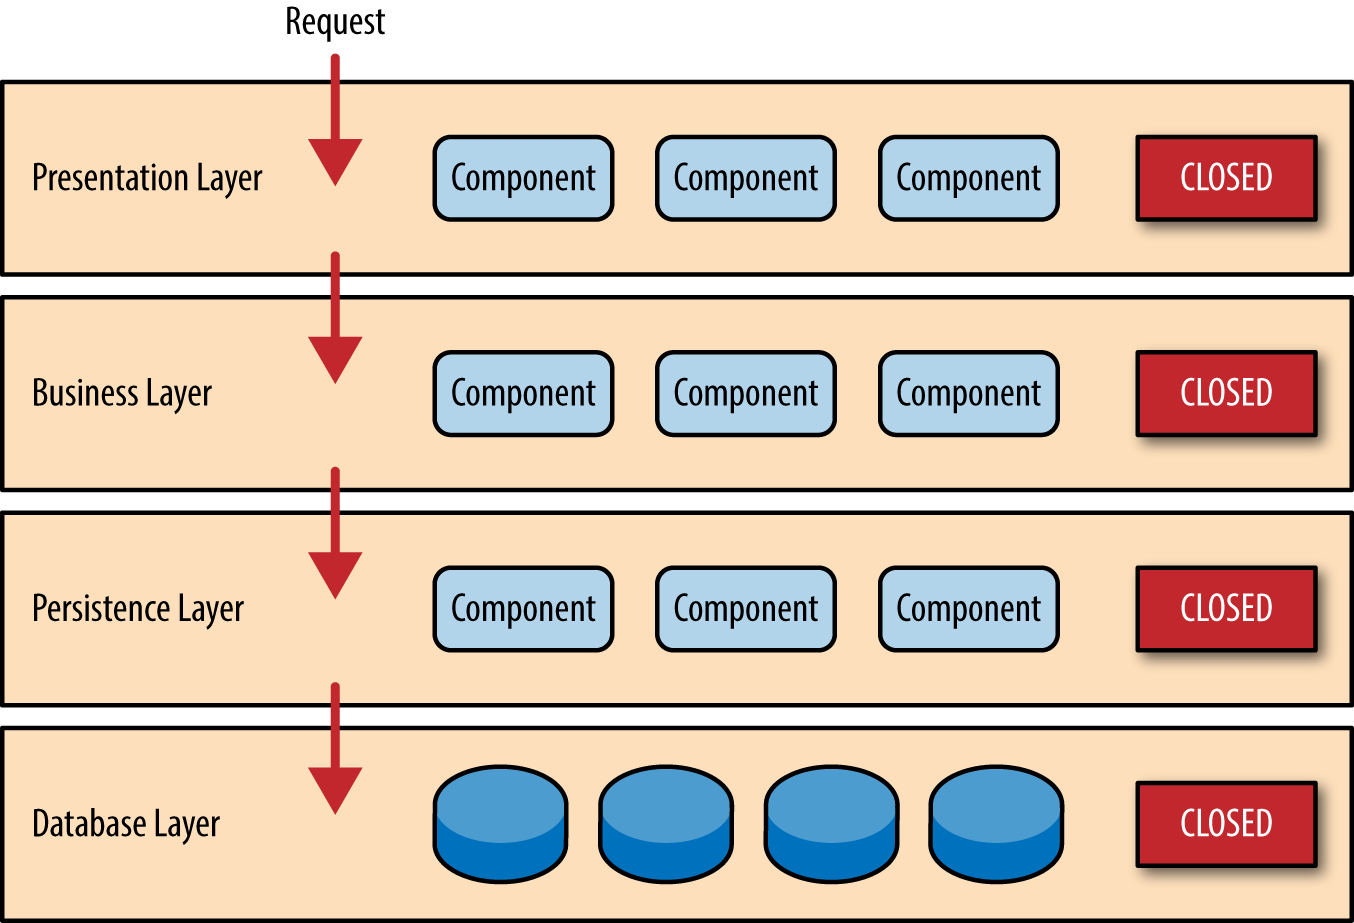
\includegraphics[width=.7\linewidth]{kapitel/problemloesung/implementierung/_img/dataflow-overview-01}
	\caption[Layered Architecture]{Layered Architecture \cite{oreilly-layered-arch}}
	\label{fig:layeredArchitecture}
\end{figure}


\begin{itemize}
  \item \emph{controller}: Dieses Package stellt alle Klassen bereit, welche direkt vom Benutzer angesprochen werden. Typischerweise handelt es sich zumindest im implementierten Stack um Rest-Schnittstellen, aber auch andere Typen (Soap, etc.) bieten entsprechende Implementierung an. Klassen dieses Packages werden allgemeinhin als Controller bezeichnet und bilden eine erste Interaktionsschicht, welche keinerlei Business-Logik enthält. Bei diesem Package handelt es sich um einen Teil des Presentation-Layers. Die Daten werden angenommen aber nicht direkt verarbeitet. Dies geschieht in sogenannten Services, die spezifische Funktionalität implementieren. Controller dienen hierbei als ein Verteiler der eingehenden Nachrichten an diese Services. Die Service-Instanzen werden den Controllern über den Spring-Context mittels Dependency Injection \todo{checken ob dependency injection irgendwo schon erklärt wurde}bereitgestellt, sodass sich der Entwickler selbst sich nicht mit der Instanziierung etc. zu beschäftigen braucht. 

  \item \emph{service}: Dieses Package enthält ausschließlich Service-Implementierungen. Ein Service stellt einen logischen Funktionsbaustein der Anwendung dar und kann über den Spring-Context bereitgestellt werden.

  \item \emph{repository}: Spring bietet über entsprechende Dependency-Starter-Konfigurationen die JPA Implementierung \emph{Hibernate} als nativen Support für die Anbindung an eine Datenbank. Dieses Package enthält Interfaces welche die Treiberschnittstelle beerben. Mithilfe spezifizierter Namenskonventionen ist es möglich Methodensignaturen für Datenbankanfragen zu gestalten. Das Framework generiert hieraus die entsprechenden SQL-Abfragen.

  \item \emph{config}: Klassen dieses Packages konfigurieren instanziieren beziehungsweise konfigurieren Spring-Beans. Es gibt bei vielen voreingestellten Spring-Komponenten die Möglichkeit Beans über Annotations in der implementierenden Klasse zu erzeugen, in bestimmten Situation wird jedoch Zugriff auf die Instanz selbst zum Initialisierungszeitpunkt gebraucht um entsprechende Konfigurationsschritte zu unternehmen. Dies geschieht standardmäßig in diesem Package.

  \item \emph{model}: Klassen, welche lediglich zum Abbilden bestimmter Datensätze genutzt werden, residieren in diesem Package. Hierbei ist es irrelevant ob es sich um JPA-Entitäten oder herkömmliche POJOs handelt.

  \item \emph{properties}: Spring bietet die Möglichkeit Daten aus den Konfigurationsdateien innerhalb der Resources direkt in den Application-Context zu laden.
  
  \item \emph{utils}: Klassen, die lediglich mit Business-Logik gefüllt sind und nicht vom Spring-Container verwaltet werden, sondern direkt im Programmcode instanziiert oder aufgerufen werden, residieren in diesem Package.
  
  \item \emph{resources}: Die genutzte Verbindungs-Konfiguration zwischen Komponenten des Stacks werden innerhalb der \emph{.properties} Dateien verwaltet. Es ist möglich auf diese Information über den Dependency-Injection-Mechanismus innerhalb der Klassen zuzugreifen.

\end{itemize}
\paragraph{Programmfluss}
Im folgenden UML-Diagramm (siehe Abbildung \ref{fig:supplierUml}) wurden ein Teil der Klassen des Suppliers dargestellt. Es wurde sich hierbei auf die wesentlichen Logikbausteine konzentriert. 

\begin{figure}[ht!]
	\centering
	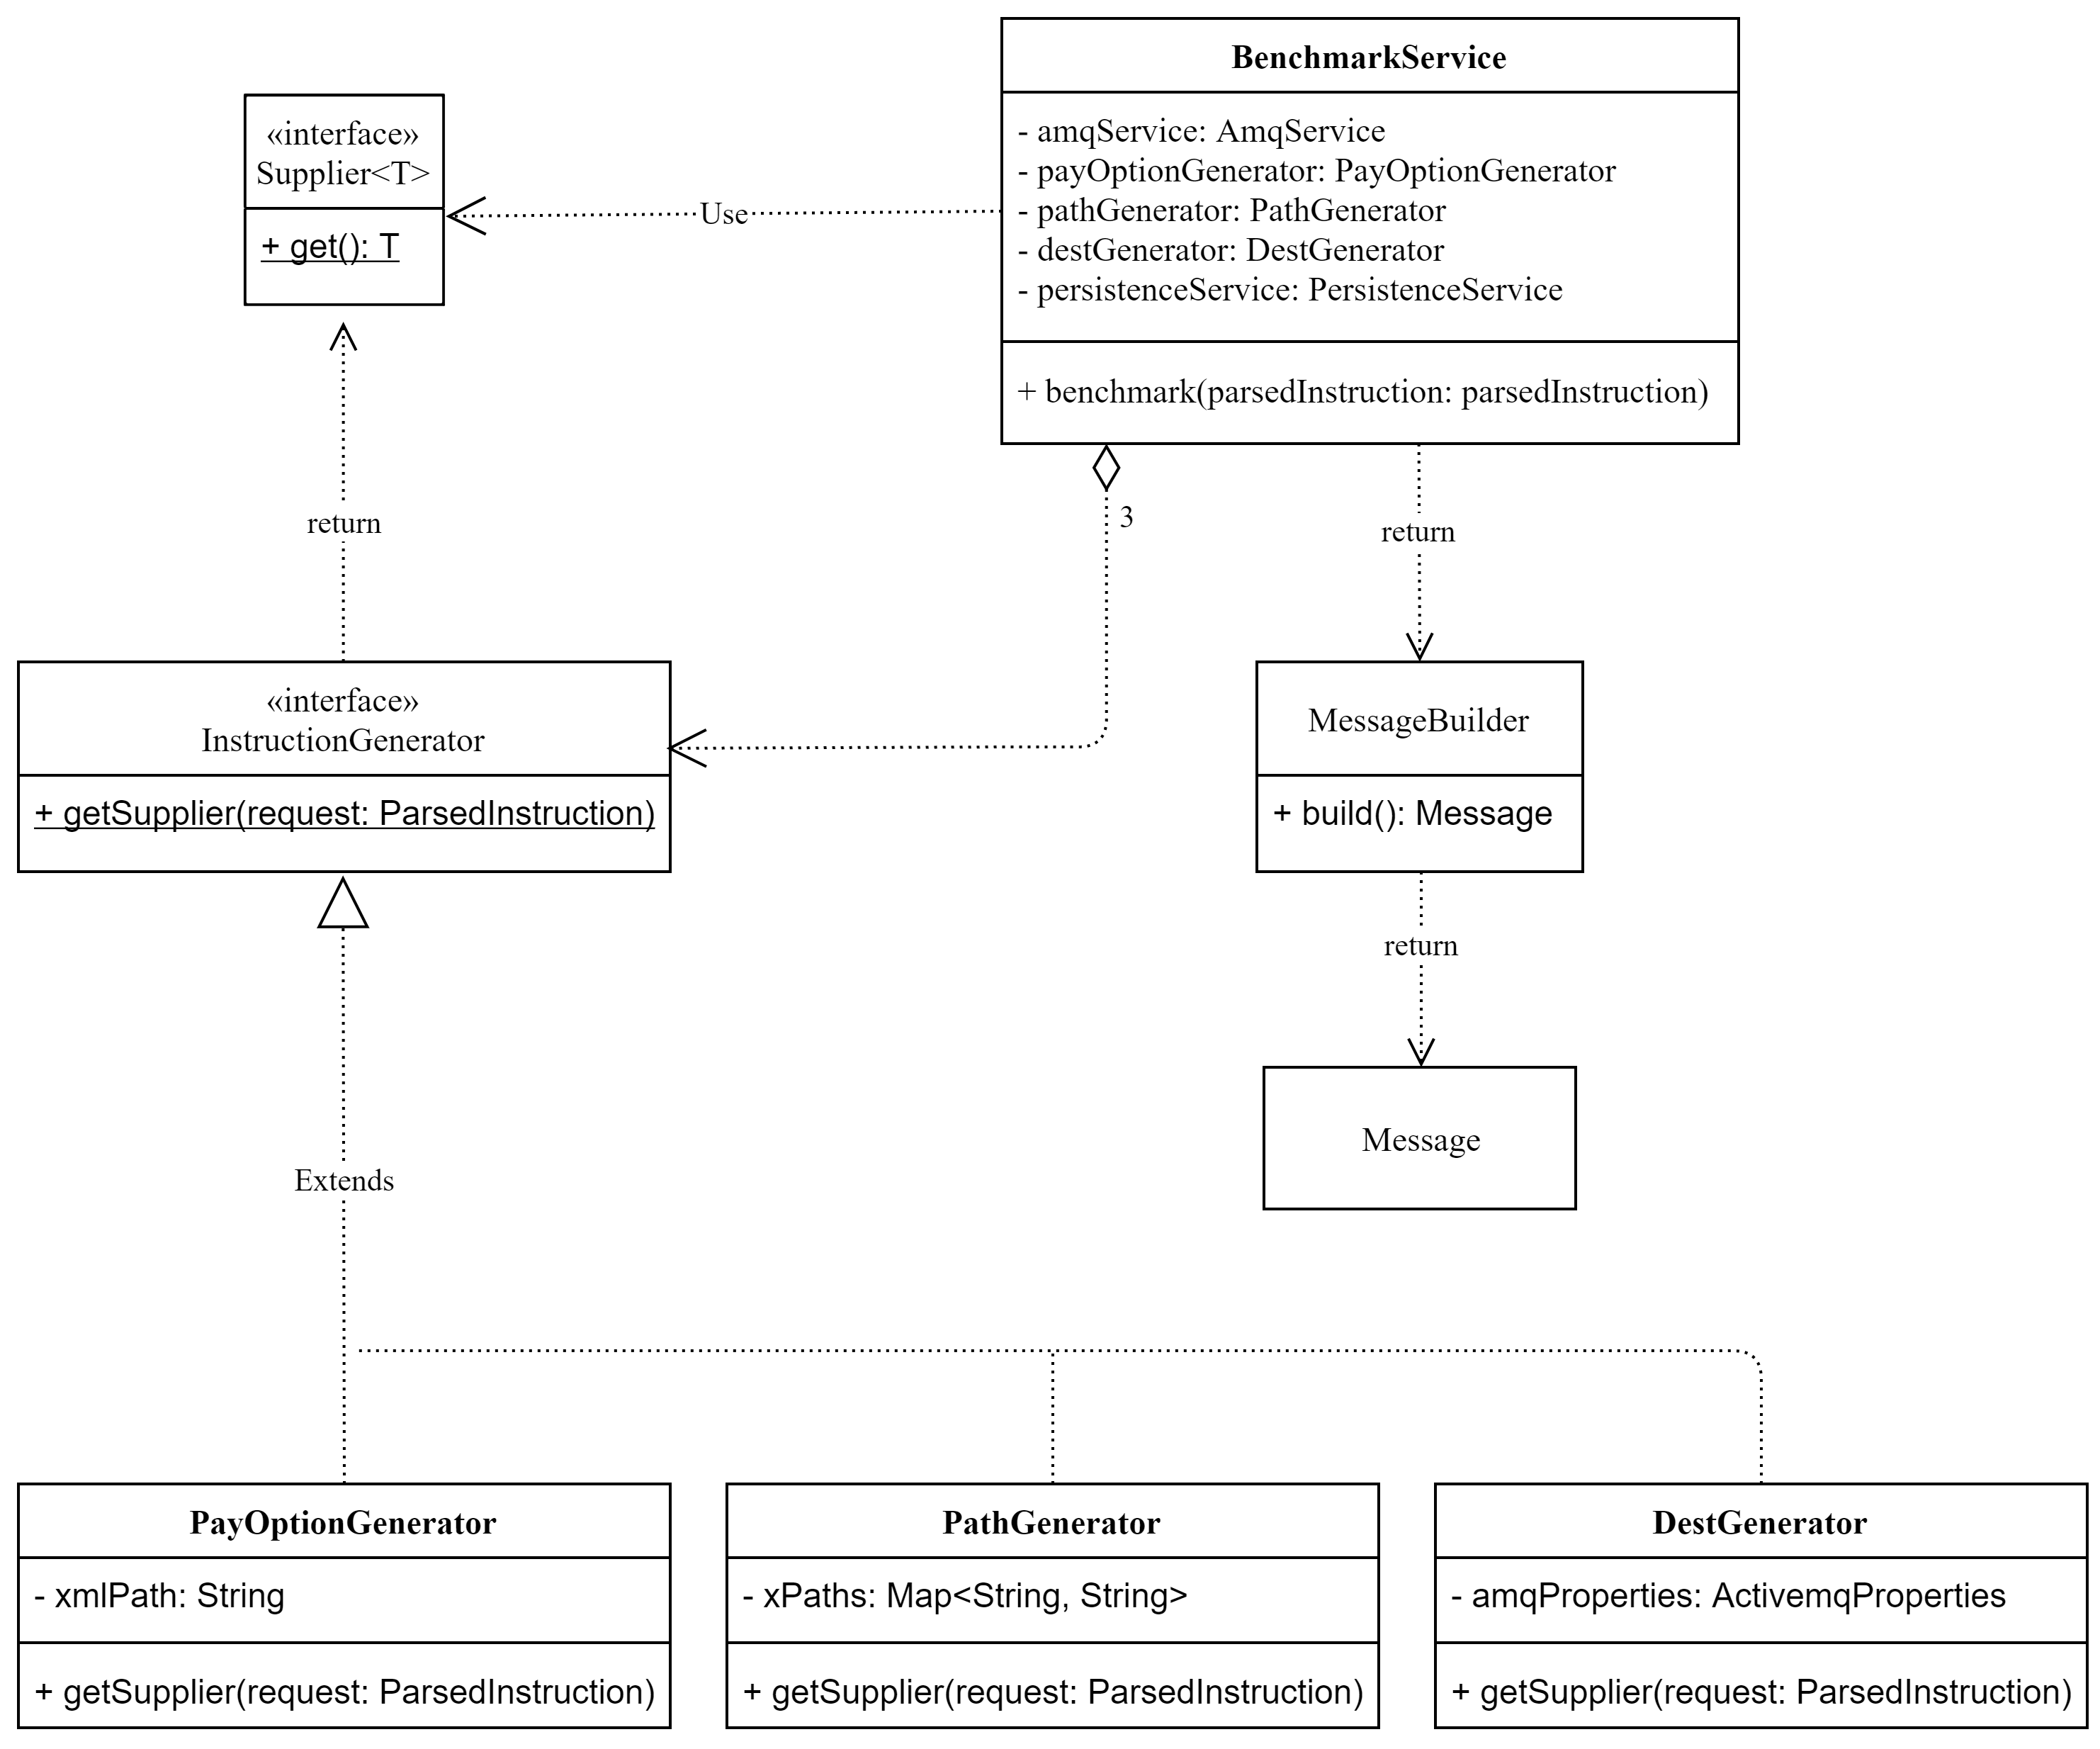
\includegraphics[width=\linewidth]{kapitel/problemloesung/implementierung/_img/supplier-uml}
	\caption[Backend Supplier UML]{Backend Supplier UML}
	\label{fig:supplierUml}
\end{figure}

Es gibt im primär zwei Einstiegspunkte für den Programmfluss. Der Benutzer möchte mithilfe der Benutzeroberfläche oder eines \emph{curl}-Aufrufs neue Nachrichten generieren, oder es wird auf die Dateiinhalte, die einer Grammatik folgen zurückgegriffen. Bei beiden Endpunkten wird im Controller eine Instanz vom Typ \emph{ParsedInstruction} erstellt. Diese enthält alle relevanten Informationen, die vom verarbeitenden \emph{BenchmarkService} gebraucht werden. Bei der Api-Anfrage durch den Curl-Aufruf lässt sich das Instanziieren direkt über das Parsen vom empfangenen Json umsetzen, während bei der Grammatik ein weiterer Service (\emph{RequestParserService}) verwendet wird, der aus der erhaltenen Grammatik diverse \emph{ParsedInstruction} Instanzen erstellt.

Wie im UML-Diagramm zu erkennen, werden aus der erhaltenen Instruktionsinstanz über verschiedene Generator-Implementierungen diverse Callbacks erstellt, die zum Absetzen der Nachrichten in das System genutzt werden. Ein Auszug des zugrunde liegenden Codes folgt in Listing \ref{lst:supplierServiceImpl};

\begin{minipage}{\linewidth}
\begin{lstlisting}[style=javaStyle,caption={Supplier - Service},label=lst:supplierServiceImpl]
  
      ...

      // create generator instances
      Supplier<String> xPathSupplier = pathGenerator.getSupplier(parsedInstruction);
      Supplier<String> paymentSupplier = payOptionGenerator.getSupplier(parsedInstruction);
      Supplier<String> destinationSupplier = destGenerator.getSupplier(parsedInstruction);
      BiConsumer<PaymentMessage, Supplier<String>> amqConsumer =
              amqService.getConsumer(sessionIsTransacted);

      ...

      for (int i = 0; i < parsedInstruction.getMessageCnt(); i++) {

          // use generator instances to dynamically create message
          PaymentMessage payment = PaymentMessage.builder()
                  .batchId(batchId)
                  .xPath(xPathSupplier.get())
                  .content(paymentSupplier.get())
                  .sentTimestamp(now())
                  .build();

          amqConsumer.accept(payment, destinationSupplier);

          Thread.sleep(durationMillis);
      }
  }

  ...
  
\end{lstlisting}
\end{minipage}

In dem beschriebenen Listing ist zu erkennen, wie diese Generatoren genutzt werden. Sie extrahieren aus der gegebenen Instruktionsinstanz die jeweils relevanten Werte für ihren Anwendungsfall (Zeile 5 -- 9) und können bei der Erstellung der Nachrichten als Callback verwendet werden, und dynamisch neue Werte erstellen (Zeile 16 -- 21). Der Grund warum hierbei auf diese Callback-Struktur zurückgegriffen wurde, ist der, dass die gegebenen Werte in der Instruktion selbst als Instruktionen verstanden werden sollen.
\paragraph{Beispiel xPathSupplier} 
Der XPath gibt an, welches XML-Element bei der Verarbeitung durch den Konsumer im Detail extrahiert werden soll (bspw. IBAN, Betrag etc.). Es ist jedoch auch möglich, dass der Benutzer bei der API-Anfrage hierbei keinen genauen XPath angibt sondern möchte, dass hierbei ein beliebiges Element extrahiert werden soll. Dazu wird der Wert "\emph{Randomize}" in die Instruktion eingetragen. Dies ist sinnvoll um etwas Variation in die spätere Verarbeitung zu bekommen um bessere Messwerte erzielen zu könnnen. Im System wurden hierfür beispielhaft einige XPath Pfade manuell hinterlegt. Der Supplier hat intern Zugriff auf diese Sammlung. Je nachdem ob ein spezifischer Wert ausgegeben werden oder dieser variieren soll, wird stets der selbe Wert oder aber unterschiedliche Werte ausgegeben. Ähnliches gilt für die anderen verfügbaren Generator-Instanzen.

\subsection{Konsumer-Komponente}

Im folgenden UML-Diagramm ist die grundlegende Klassenstruktur der beteiligten Logikbausteine des Spring-Konsumenten zu erkennen. Da das Node.js-Projekt einen sehr ähnlichen Aufbau besitzt, wird im Folgenden lediglich der Ablauf der Spring Komponente zusammengefasst. Sämtliche Informationen lassen sich jedoch nahtlos auf die Node.js-Umgebung übertragen. 

\begin{figure}[ht!]
	\centering
	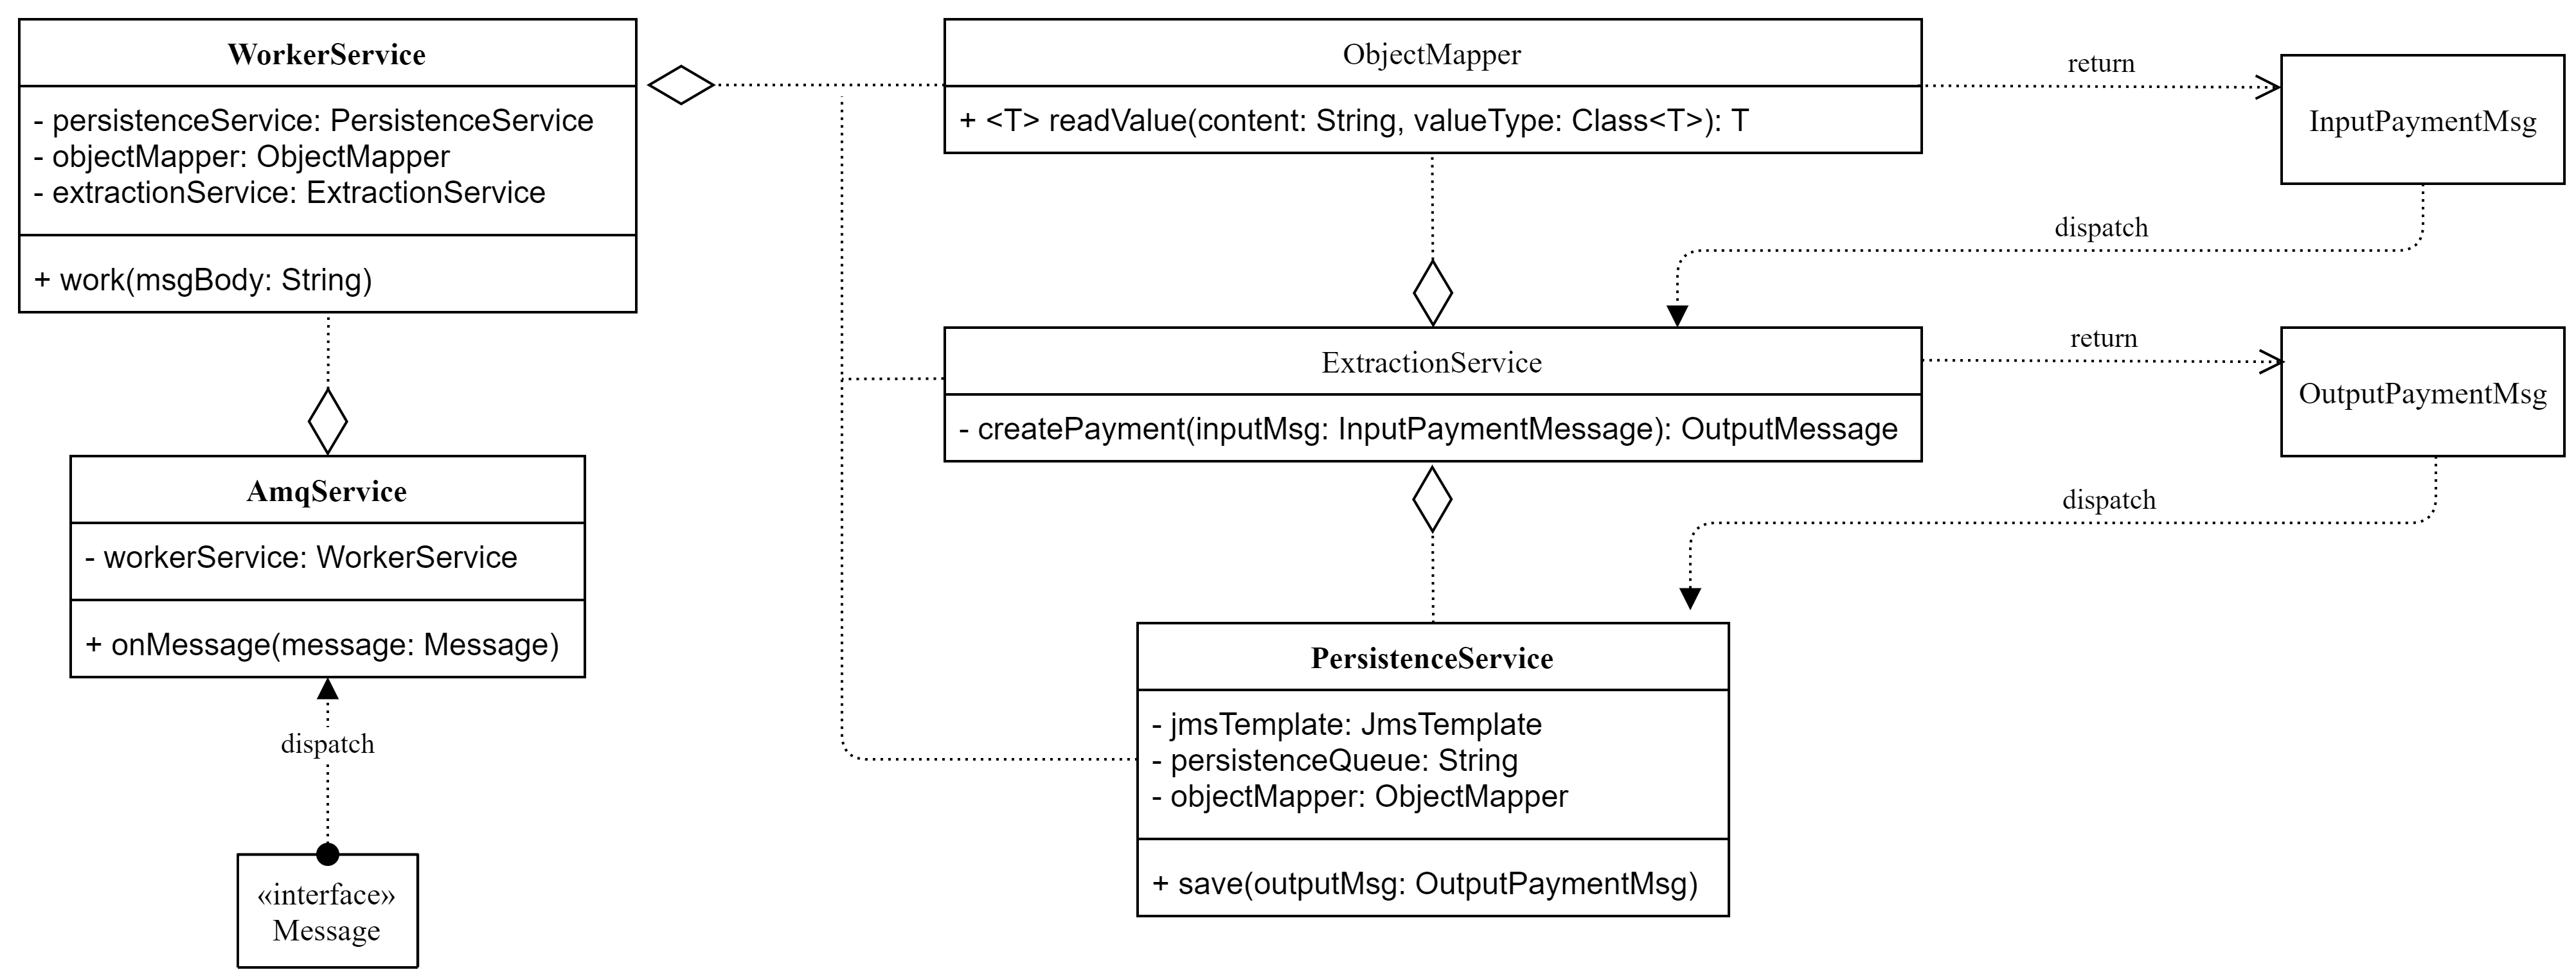
\includegraphics[width=\linewidth]{kapitel/problemloesung/implementierung/_img/consumer-uml}
	\caption[Consumer UML]{Consumer UML}
	\label{fig:consumerUml}
\end{figure}

Der Einstiegspunkt für den Spring-Konsumenten stellt der \emph{AmqService} dar. Nachrichten werden mithilfe dieser Komponente aus der Warteschlange des ActiveMq Brokers ausgelesen und an den \emph{WorkerService} delegiert. Über eine \emph{ObjectMapper} Instanz wird aus dem übergebenen String eine Objektinstanz eines Datenobjektes (\emph{InputPaymentMessage}) geniert (siehe Listing \ref{lst:consumerLogic}). Dieses Objekt wird an einen weiteren Service übergeben, der ein Element entsprechend der Vorgaben im Datenobjekt extrahiert. Wenn das zugrunde liegende XML nicht XSD konform ist oder das Element zum spezifizierten Pfad nicht gefunden werden kann, wird eine Null-Referenz ausgegeben. Es folgt ein Nullcheck bevor die Nachricht der Persistenzschicht übergeben wird.

\begin{minipage}{\linewidth}
\begin{lstlisting}[style=javaStyle,caption={WorkerService - Konsumer Logik},label=lst:consumerLogic]

  ...

  @SneakyThrows
  public void work(String msgBody) {
    InputPaymentMsg inputMessage = objectMapper.readValue(msgBody, InputPaymentMsg.class);
    OutputPaymentMsg outputMessage = extractionService.createPayment(inputMessage);
    if (outputMessage != null) {
      persistenceService.save(outputMessage);
    }
    Thread.sleep(3000);
  }

  ...

\end{lstlisting}
\end{minipage}


\subsection{Prometheus}

\paragraph{Regelsatz für Skalierung}
Die Prometheus ist eine Komponente, die zum Monitoring genutzt werden kann (siehe Abschnitt \ref{ss:prometheus}). Für dieses Projekt musste diese lediglich derartig konfiguriert werden, dass entsprechende alerts generiert werden und an die Alter-Manager-Komponente weitergeleitet werden können. Diese Komponente informiert erst anschließend die (Proxy) Scaler Komponente. Die auszuwertenden Regeln residieren jedoch bereits in der Prometheus Komponente. Die Regeln wurden nach folgendem Schema entworfen.

\bigskip

\begin{minipage}{\linewidth}
\begin{tabularx}
  {\textwidth}
  { X | X | X | X | X }
  \toprule
      \centering \hspace{4mm} \uline{QL3} \newline \footnotesize \textit{QB2 \textless{} MC} 
    & \centering \hspace{4mm} UP \newline \footnotesize \textit{abs(CB0 -- CB3)} 
    & \centering \hspace{4mm} UP \newline \footnotesize \textit{abs(CB1 -- CB3)} 
    & \centering \hspace{4mm} UP \newline \footnotesize \textit{abs(CB2 -- CB3)} 
    & \centering \hspace{4mm} OK \newline -- 
    \tabularnewline
  \hline
      \centering \hspace{4mm} \uline{QL2} \newline \footnotesize \textit{QB1 \textless{} MC $\leq$ QB2} 
    & \centering \hspace{4mm} UP \newline \footnotesize \textit{abs(CB0 -- CB2)} 
    & \centering \hspace{4mm} UP \newline \footnotesize \textit{abs(CB1 -- CB2)} 
    & \centering \hspace{4mm} OK \newline -- 
    & \centering \hspace{4mm} DOWN \newline \footnotesize \textit{abs(CB2 -- CB3)} 
    \tabularnewline
  \hline
      \centering \hspace{4mm} \uline{QL1} \newline \footnotesize \textit{QB0 \textless{} MC $\leq$ QB1} 
    & \centering \hspace{4mm} UP \newline \footnotesize \textit{abs(CB0 -- CB1)} 
    & \centering \hspace{4mm} OK \newline -- 
    & \centering \hspace{4mm} DOWN \newline \footnotesize \textit{abs(CB1 -- CB2)} 
    & \centering \hspace{4mm} DOWN \newline \footnotesize \textit{abs(CB1 -- CB3)} 
    \tabularnewline
  \hline
      \centering \hspace{4mm} \uline{QL0} \newline \footnotesize \textit{MC $\leq$ QB0} 
    & \centering \hspace{4mm} OK \newline -- 
    & \centering \hspace{4mm} DOWN \newline \footnotesize \textit{abs(CB0 -- CB1)} 
    & \centering \hspace{4mm} DOWN \newline \footnotesize \textit{abs(CB0 -- CB2)} 
    & \centering \hspace{4mm} DOWN \newline \footnotesize \textit{abs(CB0 -- CB3)} 
    \tabularnewline
  \hline
    & \centering \hspace{4mm} \uline{CL0} \newline \footnotesize \textit{CB0 == CC} 
    & \centering \hspace{4mm} \uline{CL1} \newline \footnotesize \textit{CB0 \textless{} CC $\leq$ CB1} 
    & \centering \hspace{4mm} \uline{CL2} \newline \footnotesize \textit{CB1 \textless{} CC $\leq$ CB2} 
    & \centering \hspace{4mm} \uline{CL3} \newline \footnotesize \textit{CB2 \textless{} CC $\leq$ CB3} \tabularnewline
  \bottomrule
\end{tabularx}
\end{minipage}

\bigskip

Diese Tabelle bestimmt das Skalierungsverhalten des Systems. Aus ihr werden die Regeln für die Prometheus-Konfiguration ermittelt. Um diese Tabelle etwas anschaulicher erläutern zu können, werden die folgenden Werte für entsprechende Umgebungsvariablen angenommen. 


\begin{verbatim}
  CB0=1    CB2=10    QB0=15    QB2=100
  CB1=5    CB3=30    QB1=30
\end{verbatim}


Auf der horizontale Achse wird die aktuelle Containeranzahl eines Systems in verschiedene Zustände eingeteilt. \emph{CL0} bis \emph{Cl3} beschreibt hierbei das sogenannte \emph{Container Level}. Diese Level geben Abschnitte an in denen sich die Containeranzahl zum aktuellen Zeitpunkt befinden kann, die Grenzen wurde mithilfe von Variablen festgelegt. Die Grenzen wurden mit dem Kürzel \emph{CB0} bis \emph{CB2} versehen, dies steht für den Begriff "\emph{Container Bound}". Die aktuelle Containeranzahl (engl. \emph{container count}) selbst, wurde in der Tabelle mit \emph{CC} abgekürzt. Wenn das System zu einem betrachteten Zeitraum beispielsweise fünf Containerinstanzen einer Konsumenten-Komponente laufen (im nachfolgenden stets als \emph{Consumer-Container} bezeichent). Dann befindet sich das System im Zustand \emph{Container level 1}, da die untere Grenze des Intervals mit \emph{CB0} auf 1 und die obere Grenze auf 5 gesetzt wurde. 

Eine ähnliche Eingrenzung gibt es ebenfalls für die vertikale Achse wobei die unbeantworteten Nachrichten einer Warteschlange in einem Message-Broker betrachtet werden. Hierbei steht das \emph{QL0} bis \emph{Ql3} für das sogenannte "\emph{queue level}". Über die \emph{queue bound} (kurz \emph{QB0} bis \emph{QB3}) werden hierbei die Grenzen der Intervalle festgelegt. Wenn beispielsweise 101 uneantwortete Nachrichten in der Warteschlange residieren, befindet sich das System im Zustand \emph{QL3}, da die \emph{queue count} (kurz \emph{QC}) größer der Grenze \emph{QB2} (festgelegt auf 100) .

Aus einer Überkreuzung dieser beiden Informationen lässt sich ableiten wie das System skaliert werden soll. Um beim beschriebenen Beispiel zu bleiben, würde sich das System im Feld \emph{CL1QL3} befinden. Hierbei gibt es zu wenig Container für die gegebene Nachrichtenanzahl. Die die Containeranzahl muss demnach nach oben skaliert werden und zwar um die Differenz der beiden Container-Intervall-Grenzen \emph{CB1} und \emph{CB3}. Wenn diese Skalierung durchgeführt wurde, befindet sich das System anschließend im Zustand \emph{CL3QL3}. Die Hauptdiagonale der Tabelle beschreibt die Idealzustände, hierbei muss keinerlei weitere Skalierung vorgenommen werden. 

\label{prometheus:skalierungsmechanismus}
Ein wesentlicher Nachteil dieser Herangehensweise ist, dass das System beim Skalieren über mehrere Intervallsgrenzen hinweg mit mehreren Zellen in Berührung kommt. So befindet sich das System bei der beschriebenen Skalierung beispielsweise für einen Moment im Zustand \emph{CL2QL3}. Je nach Konfiguration des Systems schlägt diese Regel hierbei an. Es gibt mehrere Möglichkeiten dieses Problem zu umgehen. Es ist zum Beispiel möglich das zeitliche Anfrageninterval nach Steuerungsinformationen vom Broker zu erhöhen, in der Hoffnung, dass das System bereits die gezielte Containeranzahl erreicht hat, wenn die nächste Anfrage erfolgt. Dies hat allerdings zur Folge, dass das System generell sehr lange braucht um zu erkennen, ob eine Skalierung bei der nächsten Aktion nötig ist oder nicht. Da dies einen sehr inpraktikabler Ansatz darstellt, wurde diese Verantwortlichkeit an den Proxy-Scaler übergeben. Da diese Komponente die tatsächlichen Skalierungsanfragen an die Docker-Scaler Api navigiert, ist sie ebenfalls in der Lage entsprechende Nachrichten zurückzuhalten, wenn klar ist, dass es sich hierbei lediglich um einen "\emph{Fehlalarm}" handelt, bei dem lediglich eine Skalierungsstufe während eines bereits laufenden Prozesses durchlaufen wird. 

Ein Satz Sonderregeln, die bisher nicht erwähnt wurden, betreffen den Initialisierungszustand. Hierbei wird geprüft ob die Minimalanzahl von Containern läuft. Falls dies nicht der Fall sein sollte, wird eine Skalierungsanfrage mit genau dieser Anzahl generiert. 


\paragraph{Konfiguration}

\begin{lstlisting}[style=bashStyle,caption={Umgebungsvariablen - Prometheus Regelsatz},label=lst:envMatrix]
  groups:
  - name: springScaleAlert
    rules:
      - alert: spring_baseline
        expr: >
          org_apache_activemq_Broker_ConsumerCount{
            brokerName="localhost",
            destinationName="${AMQ_SPRING_QUEUE_NAME}", 
            destinationType="Queue",
            instance="activemq:8080", 
            job="services"
          } < ${SCALING_CB0} 

  ...

\end{lstlisting}

Dieser Ausschnitt aus dem hinterlegten Regelwerk stellt die als letztes erwähnte Sonderregel für die minimal Containeranzahl. Hiermit wird beispielhaft beschrieben wie die erläuterten Regeln aus der Tabelle kodiert werden. Das Schlüsselwort \emph{groups} dient lediglich dazu verwandte Regeln zusammenzufassen. Der Rest ist selbsterklärend, erwähnenswert ist lediglich, dass die Wert des Schlüssels \emph{alert} in dieser Form wortwörtlich an den Alertmanager weitergeleitet und dort entsprechend verarbeitet wird.

Im folgenden Listing ist die Dateistruktur der Konfigurationsdateien von Prometheus dargestellt.

\begin{lstlisting}[style=bashStyle,caption={Umgebungsvariablen - Prometheus Regelsatz},label=lst:envMatrix]
  $ tree stack/data/prometheus/ --charset=ascii
  stack/data/prometheus/
  |-- alert-unparsed.yml
  |-- alert.yml
  |-- prometheus.yml
  `-- targets
      `-- alertmanager.json
\end{lstlisting}

In der Datei "\emph{alert-unparsed.yml}" werden die Regeln nach der bisher beschriebenen Struktur abgelegt. Hierbei wurden keinerlei festen Werte für die Intervallgrenzen eingesetzt. Zur Laufzeit der Komponente ist dies allerdings nicht zulässig. Um dennoch die Flexibilität des Formats mit Umgebungsvariablen nutzen zu können wurde ein Skript verfasst, das vor dem Starten der Komponente ausgeführt wird und die Datei "\emph{alert.yml}" generiert. In der "\emph{prometheus.yml}" Datei befindet sich ein Eintrag, der dem System mitteilt, dass diese generierte Datei für die Regelauswertung verwendet werden soll. In der \emph{prometheus.yml} Datei befinden sich ansonsten weitere Einstellungen bezüglich des Scraping Intervalls, der Adressierung der zu überwachenden Komponenten sowie die Angabe des Namens des Alert-Managers. Die komplette Konfigurationsdatei befindet sich im Anhang (siehe Listing \ref{anh:prometheusYml}).

Der Ordner \emph{target} enthält die Routing Konfiguration für die Anbindung der generierten Alerts zur Alert-Manager-Komponente.

\subsection{Alter-Manager}
Diese Komponente ist in diesem Projekt sehr einfach gehalten. Es wird lediglich ein Webhook erstellt an den erhaltene Alerts ohne jegliche Modifikation weitergeleitet werden. Im Anhang wurde die komplette Konfiguration der Komponente aufgerführt (siehe Listing lst:alertManConfig).


\subsection{Scaler Proxy}

Im folgenden UML-Diagramm (siehe Abbildung \ref{fig:proxyScalerUml}) wird die grundlegende Klassenstruktur der Scaler-Proxy-Komponente zusammengefasst. 

\begin{figure}[ht!]
	\centering
	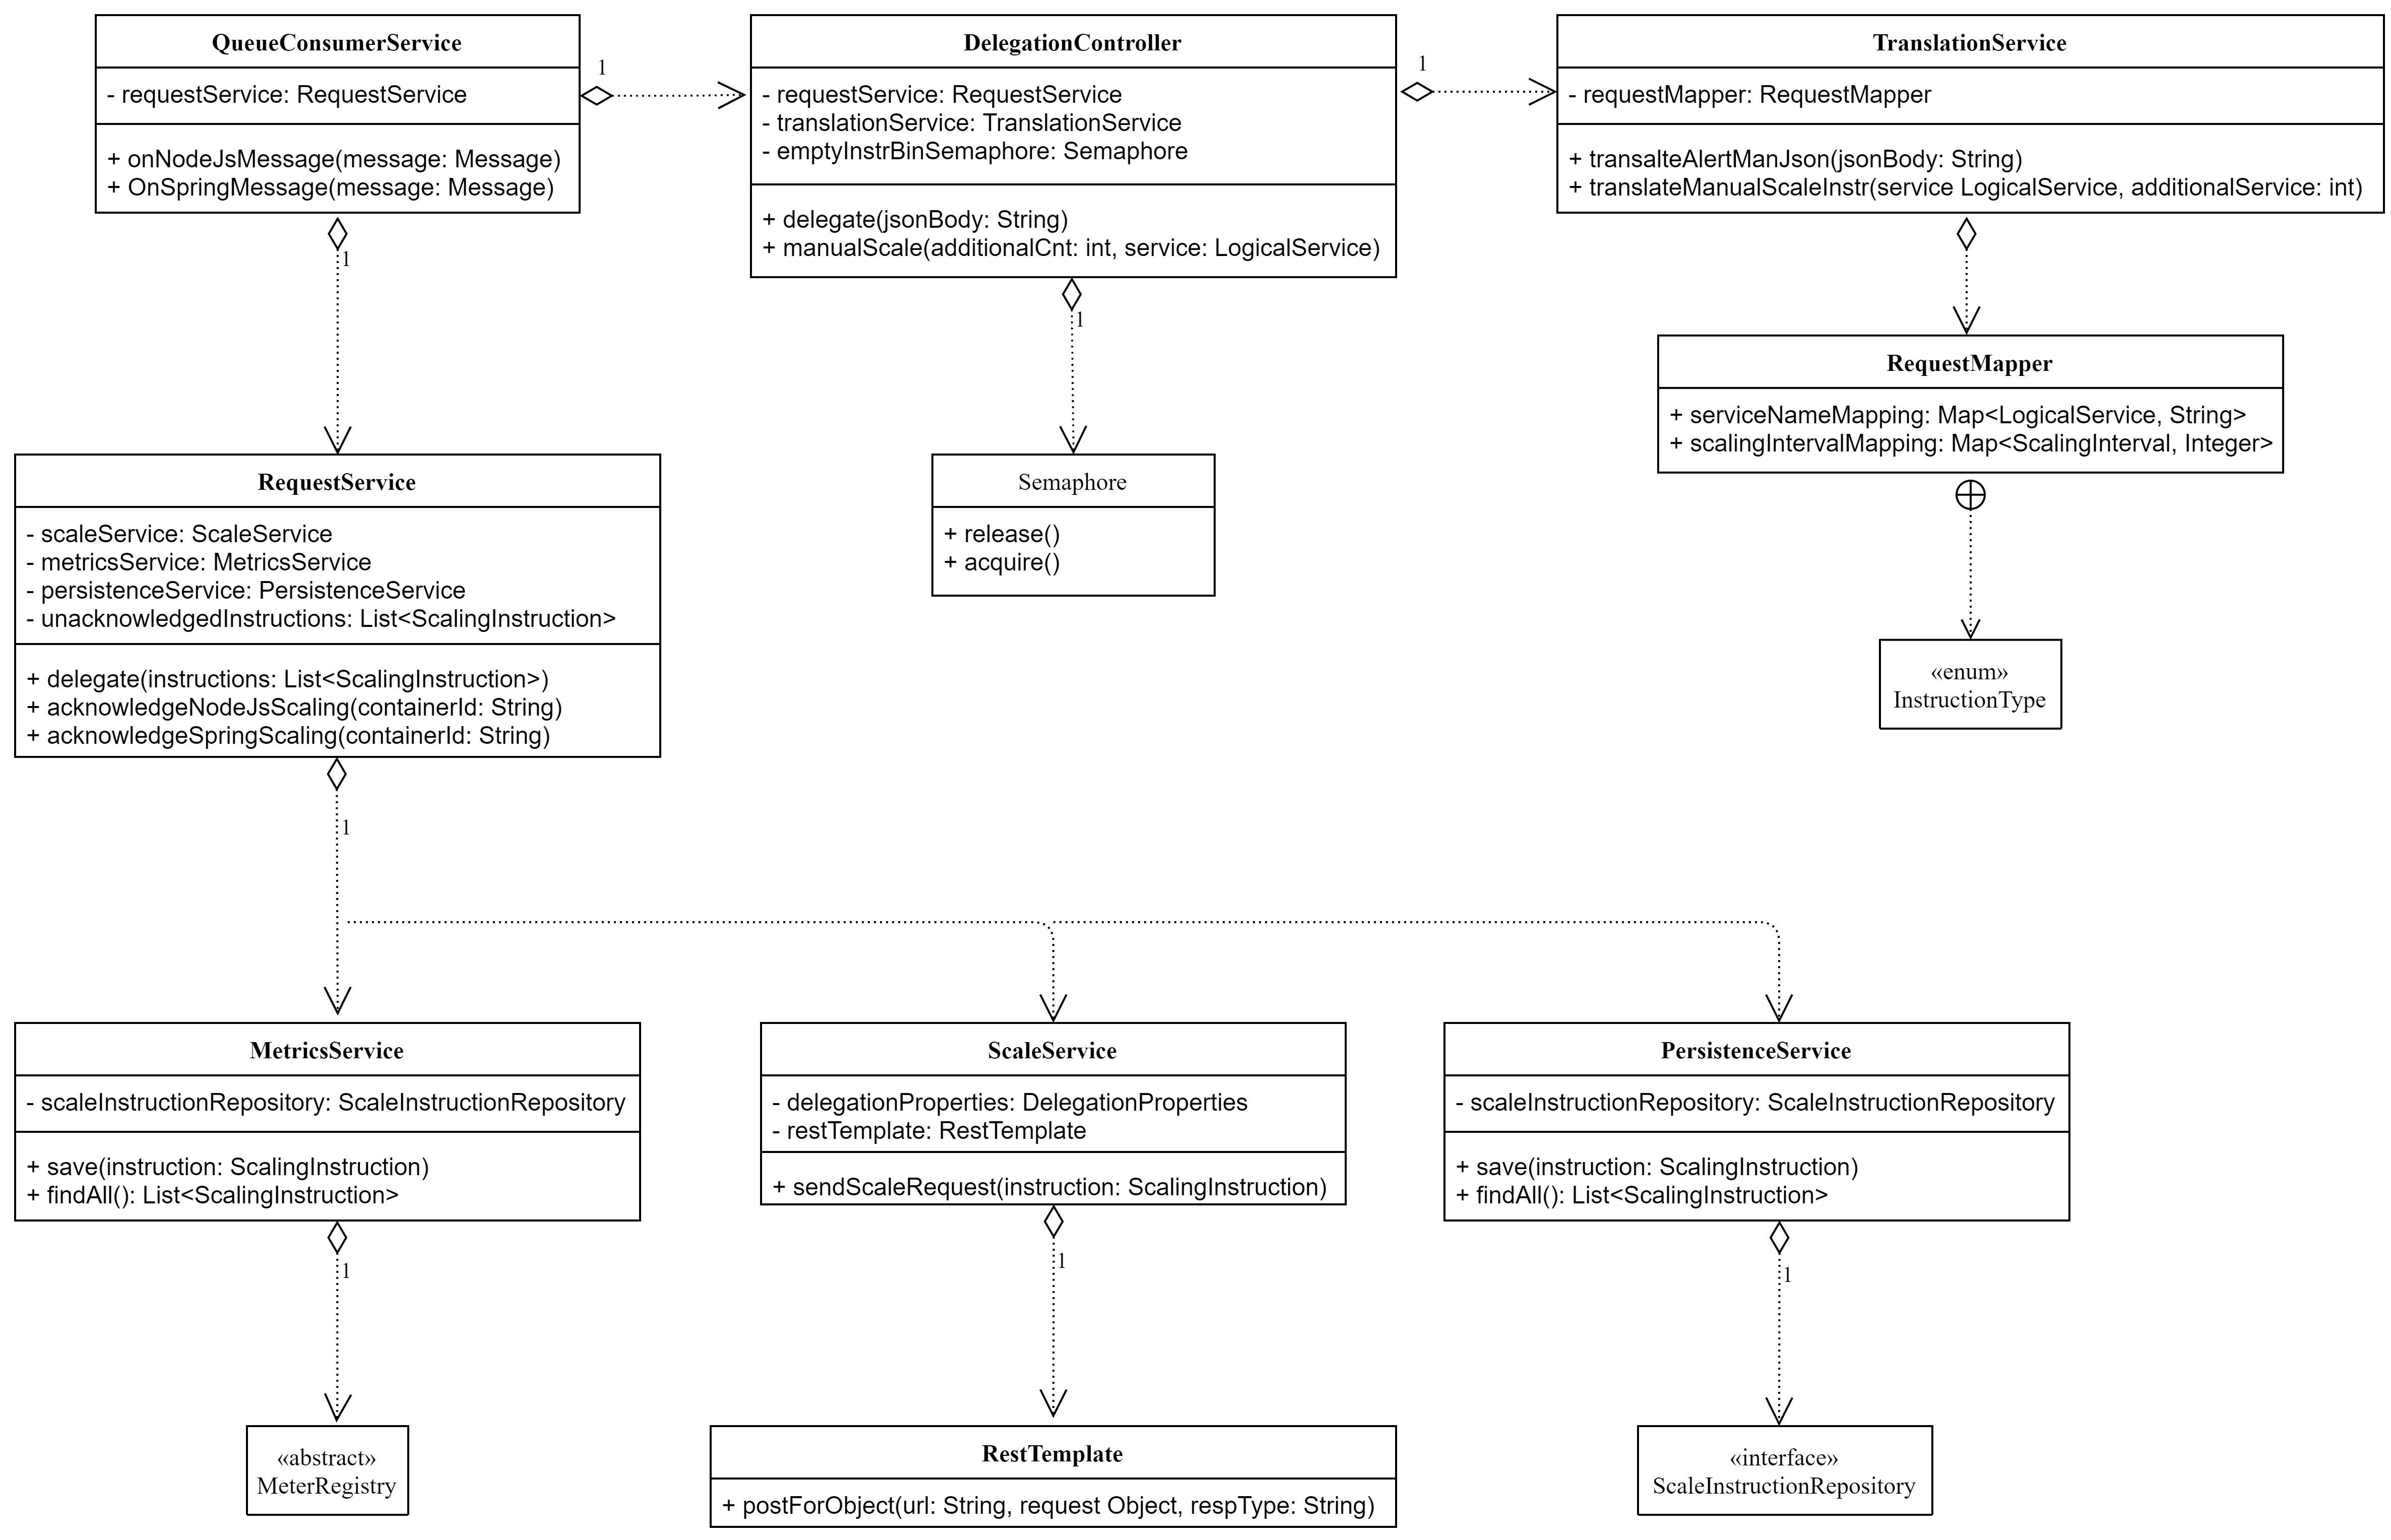
\includegraphics[width=\linewidth]{kapitel/problemloesung/implementierung/_img/scaler-proxy-uml}
	\caption[Scaler-Proxy UML]{Scaler-Proxy UML}
	\label{fig:proxyScalerUml}
\end{figure}

Diese Komponente stellt sowohl die Funktionalität bereit Alerts vom Alert-Manager als auch direkte Skalierungsanfragen vom Benutzer selbst anzunehmen. Für beide Szenarien gibt es einen entsprechenden Endpunkt. Beide Typen von Anfragen werden intern allerdings erst in ein Zwischenformat überführt, das wiederum vom \emph{RequestService} interpretiert werden kann. Die wesentliche Kernfunktionalität dieses Services wurde in Listing \ref{lst:proxyDelegate} dargestellt. Bei der Implementierung des Regelwerks in der Prometheus-Komponente wurde erwähnt, dass es einen Mechanismus zum Skalieren über mehrere Stufen des Models von der Proxy-Komponente geben muss (siehe Abschnitt \ref{prometheus:skalierungsmechanismus}). Dies wurde in der Proxy-Komponente über ein Acknowledgement der einzelnen hochgefahrenen Container ermöglicht. Es wird intern eine Liste von Skalierungsinstruktionen verwaltet. Jeder Container, der im Zuge einer der Instruktionen gestartet wird, generiert eine Id, die diesen Container identifiziert und gibt diese dem Proxy-Service über eine Rest-Schnittstelle bekannt. Dadurch ist es möglich festzustellen, ob sich das System aktuell in einem Skalierungsprozess befindet oder nicht. Wenn nun neue Skalierungsinstruktionen eingespeist werden (zum Beispiel in einer der beschriebenen Übergangsphasen in der Tabelle), dann ist es der Komponente möglich mithilfe einer einfachen Überprüfung der Liste diese zu verwerfen (Zeile 2). Im Anschluss wird über sämtliche generierten Skalierungsinstruktionen iteriert. Die verwaltete Liste wird mit neuen Einträgen gefüllt und die Anfragen werden an die Skalierungs-API geschickt, welche als letztes Abstraktionslevel ohne weitere Funktionalität die Skalierung für den Benutzer übernimmt. 

\begin{lstlisting}[style=javaStyle,caption={Proxy Scaler - RequestService},label=lst:proxyDelegate]
  public boolean delegate(List<ScalingInstruction> instructions) {
    if (!unacknowledgedInstructions.isEmpty()) {
        return false;
    }
    boolean scaledToMinRepl = false;
    for (ScalingInstruction instruction : instructions) {
        instruction.setReceivedRequestTimestamp(now());
        if (instruction.getScalingDirection() == UP) {
            unacknowledgedInstructions.add(instruction);
        }
        scaledToMinRepl = scaledToMinRepl || scaleService.sendScaleRequest(instruction);
    }
    return scaledToMinRepl;
  }
\end{lstlisting}


\subsection{Docker-Scaler}
Dieses open source Projekt\footnote{\url{https://thomasjpfan.github.io/docker-scaler}} bietet eine Rest-Schnittstelle über die es möglich ist einen zugrunde liegenden Docker-Swarm zu skalieren. Die komplette Anfrage kann innerhalb einer einzigen POST-Anfrage abgeschickt werden. In diesem Projekt wurde hierfür der folgende Endpunkt verwendet.

\begin{itemize}
  \item URL: /v1/scale-service
  \item Methode: POST
  \item Parameter:
  \begin{itemize}
    \item service: Name des zu skalierenden Services
    \item scale: Richtung in die skaliert werden soll 
    \item by: Anzahl zusätzlichen / überflüssigen Replicas
  \end{itemize}
\end{itemize}


\subsection{Grafana}

Dieses Werkzeug wird zur Erstellung von Graphen von erhaltenen Daten verwendet. Diese Daten werden von allen relevanten Stack-Komponenten über eine einheitliche Schnittstelle bereitgestellt und im Prometheus Client gebündelt. Die Grafana-Komponenten muss hierbei lediglich die Prometheus-Komponente als \emph{Datasource} deklarieren um Zugriff auf diese Metriken zu erhalten \cite[Seite~99 ff.]{oreillyPrometheus}. In Abbildung \ref{fig:prometheusDatasource} ist diese Konfiguration in Auszügen zu erkennen. Hierbei wird im Wesentlichen die Netzwerk-Adresse und Port spezifiziert. 

\begin{figure}[ht!]
	\centering
	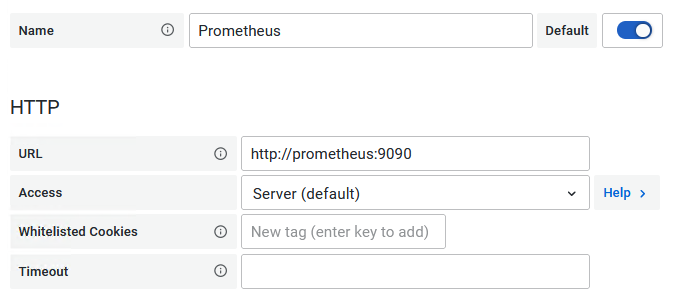
\includegraphics[width=.9\linewidth]{kapitel/problemloesung/implementierung/_img/prometheus-datasource}
	\caption[Prometheus - Datesource]{Prometheus - Datesource}
	\label{fig:prometheusDatasource}
\end{figure}

Über die in Prometheus deklarierten \emph{Targets} können die wichtigen Informationen ausgelesen werden. Die Abbildung \ref{fig:grafanaOverview} zeigt hierbei auf wie das fertige Dashboard aussieht. Die Aufnahme wurde zum Zeitpunkt der Benchmarks-Test, die als Grundlage für diese Analyse verwendet wurden, getätigt. Es lassen sich alle Metriken der Ergebnisanalyse (siehe Abschnitt \ref{} \todo{ref einbinden}) in diesem  Dashboard wiederfinden. 

\begin{figure}
	\centering
	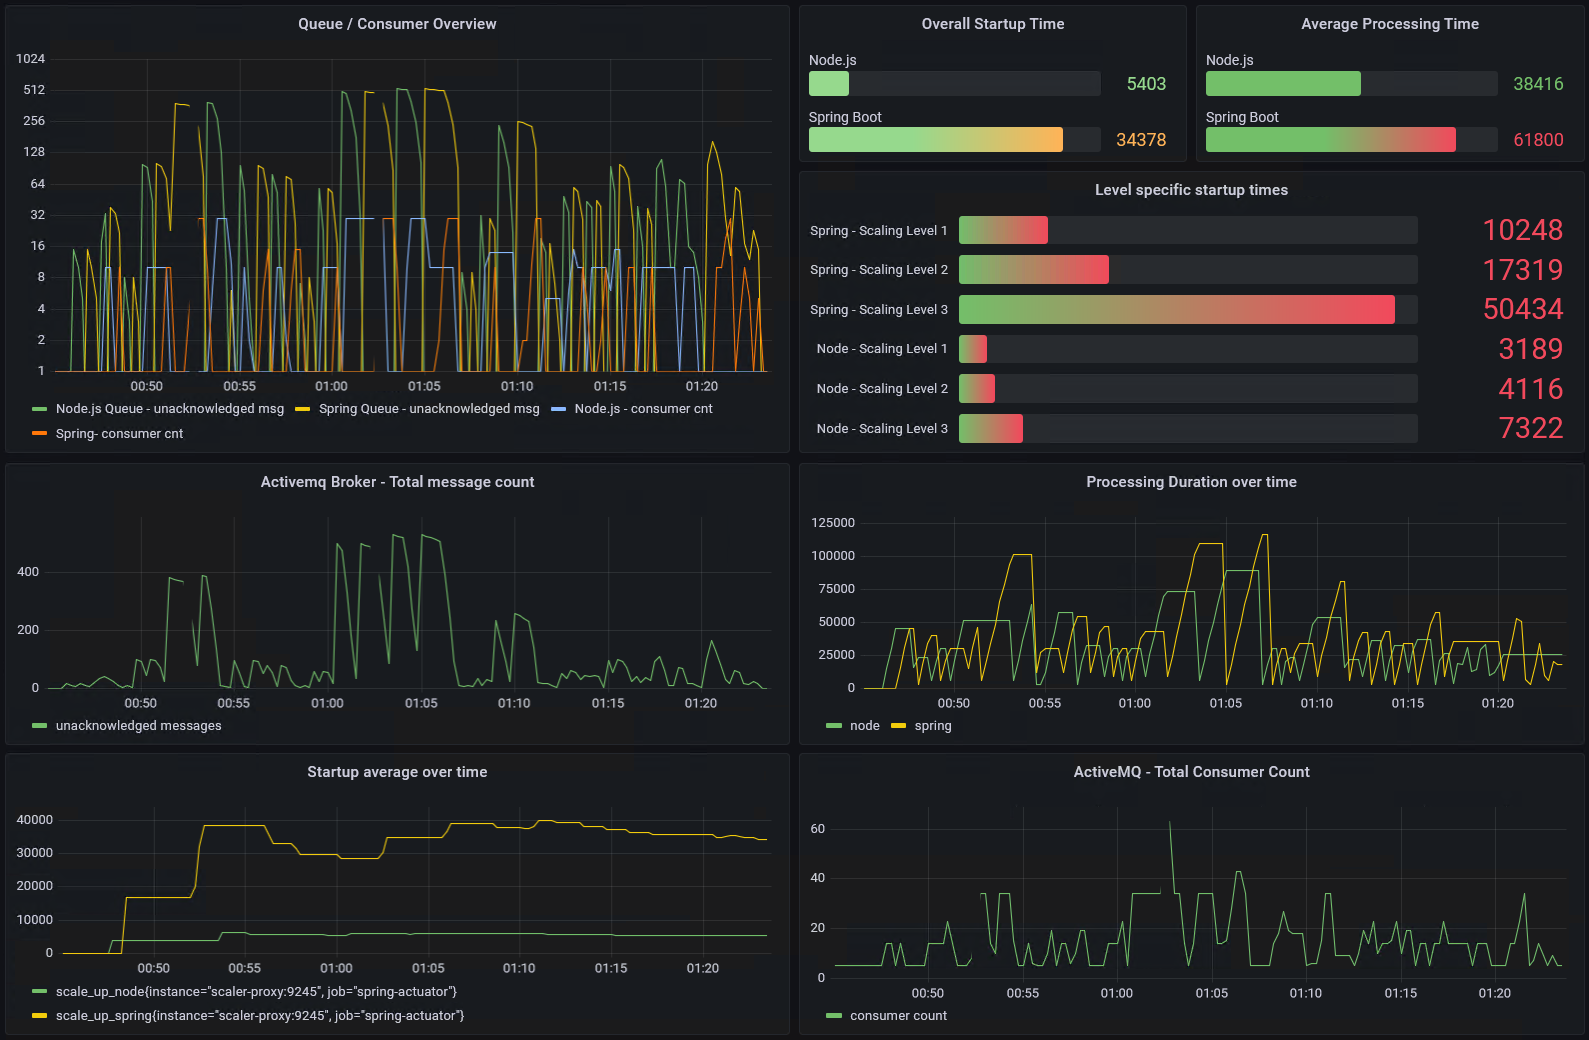
\includegraphics[width=\linewidth]{kapitel/problemloesung/implementierung/_img/grafana-dashboard-01}
	\caption[]{Grafana Dashboard}
	\label{fig:grafanaOverview}
\end{figure}

Um ein Dashboard zu erstellen, wird auf das Webinterface der Komponente selbst zugegriffen. Es gibt hierbei zwar auch die Möglichkeit Dashboards im Json-Format einzulesen sowie zu exportieren, der Einfachheit halber wurde in diesem Projekt allerdings hierrauf verzichtet. In der folgenden Abbildung ist zu erkennen, wie die Konfiguration einer Dashboard-Komponente über das Webinterface funktioniert (siehe Abbildung \ref{fig:grafanaPromQl}). 

\begin{figure}
	\centering
	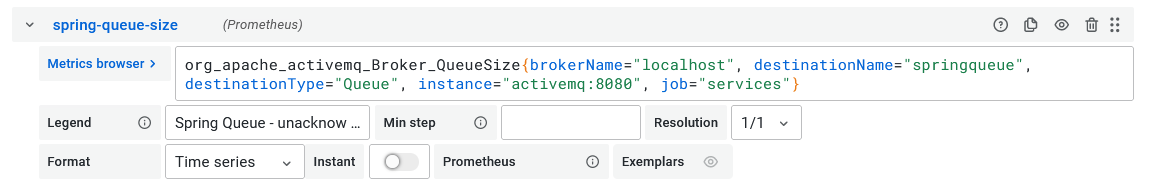
\includegraphics[width=\linewidth]{kapitel/problemloesung/implementierung/_img/grafana-promql}
	\caption[]{Grafana - Graphenkonfiguration}
	\label{fig:grafanaPromQl}
\end{figure}

Die wesentliche Hauptkomponente, die während der Konfiguration verwendet wird, stellt die Anfrage an die definierte Datasource dar (\emph{query}). Hierbei wird auf eine Anfragesprache namens \emph{PromQL} zurückgegriffen um verschiedene Metriken auslesen zu können. In der Abbildung ist beispielsweise zu erkennen, dass bei einem Messagebroker mit dem Namen "\emph{localhost}" eine Warteschlang (engl. emph{queue}) mit dem Namen "\emph{springqueue}" mit der Adresse "\emph{activemq:8080}" die aktuelle Größe der Warteschlange ausgeben soll\footnote{Die hier genutzte Anfrage lässt sich zum Beispiel bei der ActiveMq-Dokumentation nachlesen \url{https://docs.splunk.com/Observability/gdi/activemq/activemq.html}}. Diese Anfrage wird in einem konfigurierbaren Intervall wiederholt (hier alle 15 Sekunden). Es ist auch möglich mehrere Anfragen pro Graph zu definieren um mehrere Werte gegenüberzustellen sowie mehrere Anfragen zu verknüpfen. Die erhaltenen Daten werden anschließend automatisch in einem Graphen dargestellt (siehe Abbildung \ref{fig:graphEx}). 

\begin{figure}
	\centering
	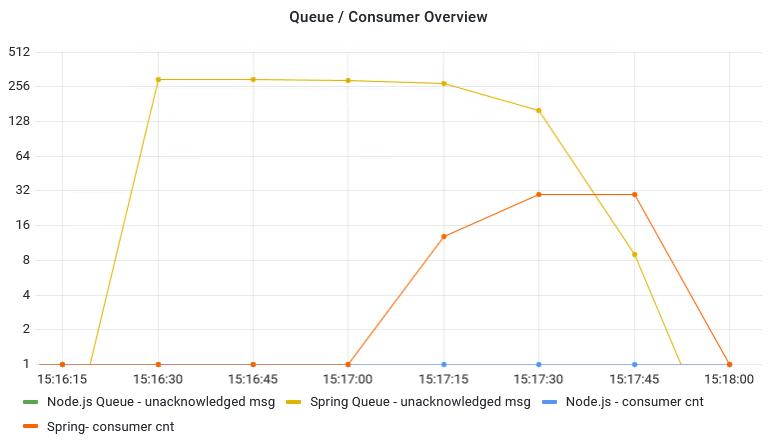
\includegraphics[width=.8\linewidth]{kapitel/problemloesung/implementierung/_img/grafana-graphExample}
	\caption[]{Grafana - Beispielhafter Graph}
	\label{fig:graphEx}
\end{figure}

In diesem Beispiel wurden eine größere Menge von Nachrichten für den Spring-Konsumenten in die Warteschlange geladen. Die unbeantworteten Nachrichten wurden hierbei in gelb dargestellt. Da zum Start der Anwendung nur ein einziger Container des Services aktiv läuft, werden im Nachhinein weitere Container hochgefahren (siehe orangene Kurve). Es ist zu erkennen, dass die Nachrichtenanzahl zu anfang sehr langsam abnimmt mit ansteigender Container anzahl jedoch immer schneller sinkt.

Die Daten hinsichtlich der Node.js Komponenten sowie die Zahlenwerte für die gemessenen Start-up-Zeiten werden ebenfalls in eigenen Dashboard-Komponenten dargestellt. Da die Konfiguration dieser, der vorgestellten allerdings deutlich ähnelt, wurde hierbei darauf verzichtet diese ebenfalls zu erläutern. Da das Dashboard im allgemeinen einen eher überprüfenden Charakter einnimmt um nachvollziehen zu können wie die letztendlichen Messwerte berechnet wurden, ist diese gesamte Komponente auch von nebensächlicher Bedeutung.


% \subsection{Buildprozess}

% % \begin{lstlisting}[language=bash]
% %  tree . -L 1
% % .
% % ├── Dockerfile
% % ├── package.json
% % ├── package-lock.json
% % ├── specification.xsd
% % ├── src
% % └── tsconfig.json
% % \end{lstlisting}
% % \todo{uncomment}

% \subsubsection{Projektübersicht}
% Das Projekt beinhaltet neben sämtlichen Quellcode-Dateien ein Dockerfile, eine package.json und eine tsconfig Konfigurationsdatei. 

% \subparagraph{Dockerfile}
% Bei dem verwendeten Dockerfile handelt es sich um eine multi-stage Konfiguration. \todo{Quellen raussuchen}

% \todo{Zeilennummern}
% \begin{lstlisting}[language=bash]
%   # stage 1 building the code
%   FROM node:10.15.3 AS builder
%   WORKDIR /usr/app
%   COPY package*.json ./
%   RUN npm install
%   COPY . .
%   RUN npm run build 
  
%   # stage 2
%   FROM node:10.15.3-alpine
%   WORKDIR /usr/app
%   COPY package*.json ./
%   RUN npm install --production
  
%   COPY --from=builder /usr/app/dist ./dist
  
%   COPY --from=builder /usr/app/schema.sql .
%   COPY --from=builder /usr/app/specification.xsd .
  
%   CMD node dist/src/index.js
% \end{lstlisting}

% \subparagraph{Typescript Konfiguration}

% \subparagraph{Quellcode}


% \begin{minipage}{\linewidth}
% \begin{lstlisting}[style=bashStyle,caption={Node.js Projektstruktur},label=lst:nodeProjStruc]
%   $ tree stack/node-consumer/ -a -L 3 --charset=ascii
%   stack/node-consumer/
%   |-- Dockerfile
%   |-- .dockerignore
%   |-- package.json
%   |-- package-lock.json
%   |-- schema.sql
%   |-- scripts
%   |   `-- buildimage.sh
%   |-- specification.xsd
%   |-- src
%   |   |-- index.ts
%   |   |-- model
%   |   |   |-- PaymentInput.ts
%   |   |   |-- PaymentMessage.ts
%   |   |   `-- ResultWrapper.ts
%   |   |-- service
%   |   |   |-- AmqService.ts
%   |   |   `-- WorkerService.ts
%   |   `-- utils
%   |       |-- ElementExtractor.ts
%   |       |-- IdGenerator.ts
%   |       `-- XsdChecker.ts
%   `-- tsconfig.json
% \end{lstlisting}
% \end{minipage}


% Die Programmlogik wurde in drei wesentliche packages aufgeteilt (siehe Listing \todo{Listing einkommentieren und referenzieren}). 

% \begin{itemize}
%   \item \emph{model}: Dieses Package beinhaltet sämtliche Datenstrukturen, die vom System zur Bearbeitung der eingehenden Nachrichten verwendet werden.
%   \item \emph{model}: Dieses Package beinhaltet sämtliche Komponenten welche logisch klar abgetrennte Aufgabe implementieren und über Schnittstellen miteinander kommunizieren. Hierbei wurde sich an der Architektur einer typischen Spring-Anwendung orientiert.
%   \item \emph{model}: Dieses Package beinhaltet sämtliche Funktionalität der abzuarbeitenden Businesslogik.
% \end{itemize}





\section{Deployment auf Containerplattform}
Nachdem im letzten Abschnitt beschrieben wurden, wie die einzelnen Stack-Komponenten implementiert wurde, wird im Folgenden auf das Deployment mithilfe von Containern im Docker Swarm Stack eingegangen.

\subsection{Build}
Um das Projekt im Komponenten-Stack als Dockercontainer zu deployen, muss in einem ersten Schritt ein Docker Image erstellt werden. Dieses kann im Anschluss als Container instanziiert werden. Zum Erstellen eines Docker-Images wird auf ein sogenannten "\emph{Dockerfile}" zurückgegriffen, das die Beschreibung des Build-Prozesses für dieses Image enthält. Da alle Spring-Projekte im Komponenten-Stack mit einem fast identischen Dockerfile versehen wurden, gilt die folgende Beschreibung in gleichem Maß für alle weiteren Spring-Projekte. \todo{Multistage Build erklären / Quelle raussuchen}

\begin{minipage}{\linewidth}
\begin{lstlisting}[style=javaStyle,caption={Supplier - Bi Consumer},label=lst:supplierParserEndpoint]
  FROM maven:3.8.1-openjdk-11 AS build
  COPY src /usr/src/app/src
  COPY pom.xml /usr/src/app
  RUN mvn -f /usr/src/app/pom.xml clean package -DskipTests

  FROM gcr.io/distroless/java
  COPY --from=build /usr/src/app/target/supplier-backend.jar /usr/app/supplier-backend.jar
  EXPOSE 9245
  ENTRYPOINT ["java","-jar","/usr/app/supplier-backend.jar"]
\end{lstlisting}
\end{minipage}

\begin{itemize}
  \item Zeile 1: Ein Dockerfile beginnt meist mit der Angabe eines sogenannten "\emph{Baseimages}". Dies kann eine minimale Linux Distribution sein, oder wie in diesem Fall ein System auf dem bereits diverse Konfigurationen definiert wurden. Bei dem verwendeten Image, wurde eine Java Runtime sowie das Buildprogramm \emph{maven} bereits vorinstalliert. Beides wird für die Ausführung des Spring-Projekts gebraucht. 
\end{itemize}







\subsection{Container Lifecycle}
\begin{itemize}
  \item Auf verschiedene Schichten eingehen
  \item Auf Ergebnisse beziehen
\end{itemize}
\subsection{Docker Swarm}

\begin{itemize}
  \item Prototypen im Detail erlaeutern
\end{itemize}


\renewcommand\theadalign{bc}
\renewcommand\theadfont{\bfseries}
\renewcommand\theadgape{\Gape[4pt]}
\renewcommand\cellgape{\Gape[4pt]}





\section{Implementierung Lasttest}
\subsection{Timeline}
\subsection{Testbedingungen}
\begin{itemize}
  \item Kommt in den Anhang
  \item hat Prof. zwar als eigenes Kapitel erwaehnt, bin mir aber nicht sicher ob das wirklich noetig ist
  \item auf welcher Hardware werden Tests durchgefuehrt?
  \item chaos monkey / Stoerfaelle erlaeutern
\end{itemize}

\begin{table}
  \centering
  \caption{Server Specs}
  \bigskip
  \begin{tabular}{ c l }
    \toprule
    Prozessor & Intel(R) Xeon(R) Gold 6226R CPU @ 2.90GHz \\
    \midrule
    Kerne & 6 Prozessoren á 16 Kerne \\
    \midrule
    RAM & 16 GB \\
    \midrule
    Storage & 150 GB \\
    \bottomrule
  \end{tabular}
\end{table}


\section{Implementierung Visualierung und Monitoring zur Unterst\"utzung der Auswertung}

% \begin{lstlisting}[language=bash]
%  tree . -L 1
% .
% ├── Dockerfile
% ├── package.json
% ├── package-lock.json
% ├── specification.xsd
% ├── src
% └── tsconfig.json
% \end{lstlisting}





\begin{itemize}
  \item 
\end{itemize}